% Created by tikzDevice version 0.9 on 2016-01-12 22:38:39
% !TEX encoding = UTF-8 Unicode
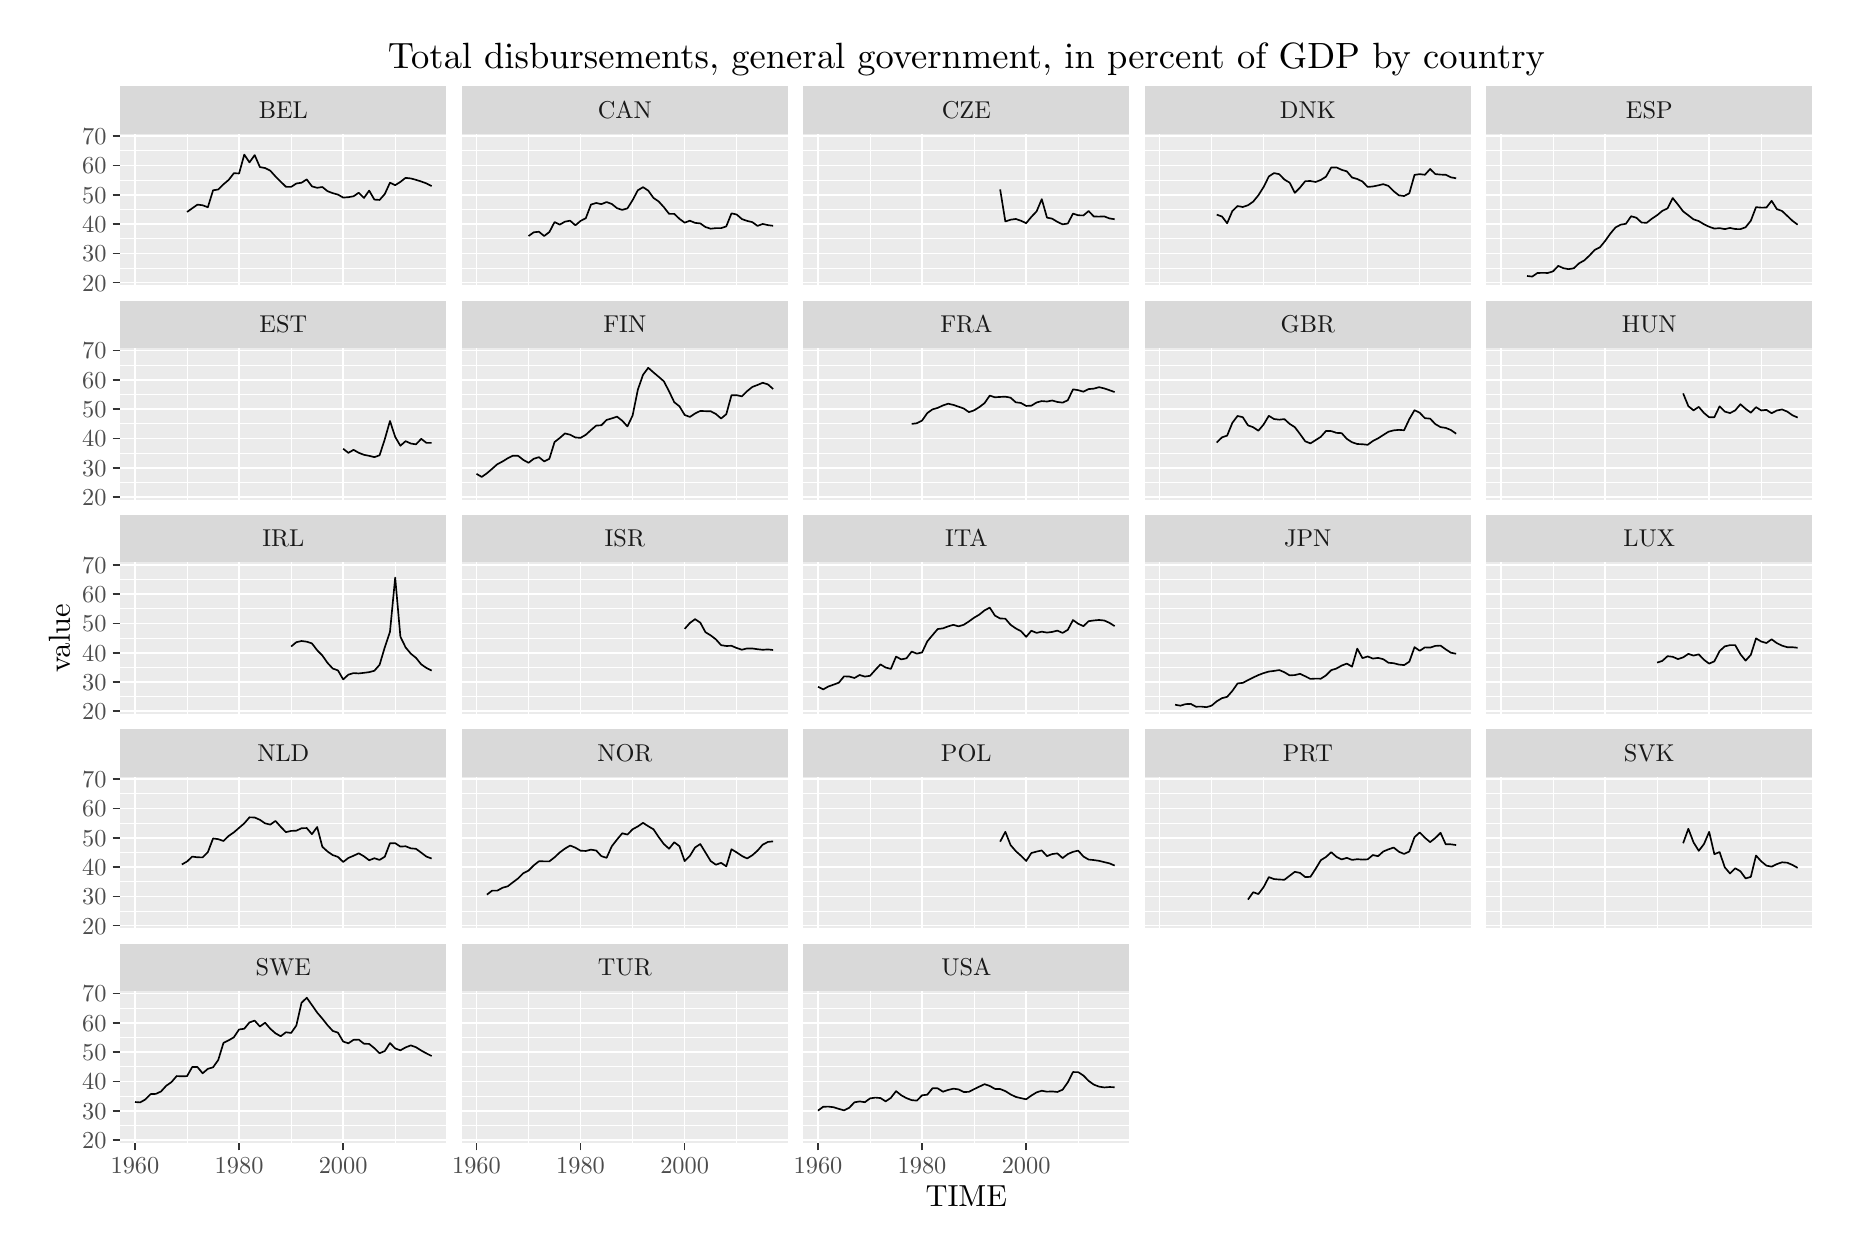
\begin{tikzpicture}[x=1pt,y=1pt]
\definecolor{fillColor}{RGB}{255,255,255}
\path[use as bounding box,fill=fillColor,fill opacity=0.00] (0,0) rectangle (650.43,433.62);
\begin{scope}
\path[clip] (  0.00,  0.00) rectangle (650.43,433.62);
\definecolor{drawColor}{RGB}{255,255,255}
\definecolor{fillColor}{RGB}{255,255,255}

\path[draw=drawColor,line width= 0.6pt,line join=round,line cap=round,fill=fillColor] (  0.00,  0.00) rectangle (650.43,433.62);
\end{scope}
\begin{scope}
\path[clip] ( 33.42,340.48) rectangle (151.33,395.37);
\definecolor{fillColor}{gray}{0.92}

\path[fill=fillColor] ( 33.42,340.48) rectangle (151.33,395.37);
\definecolor{drawColor}{RGB}{255,255,255}

\path[draw=drawColor,line width= 0.3pt,line join=round] ( 33.42,346.77) --
	(151.33,346.77);

\path[draw=drawColor,line width= 0.3pt,line join=round] ( 33.42,357.35) --
	(151.33,357.35);

\path[draw=drawColor,line width= 0.3pt,line join=round] ( 33.42,367.93) --
	(151.33,367.93);

\path[draw=drawColor,line width= 0.3pt,line join=round] ( 33.42,378.51) --
	(151.33,378.51);

\path[draw=drawColor,line width= 0.3pt,line join=round] ( 33.42,389.10) --
	(151.33,389.10);

\path[draw=drawColor,line width= 0.3pt,line join=round] ( 57.59,340.48) --
	( 57.59,395.37);

\path[draw=drawColor,line width= 0.3pt,line join=round] ( 95.20,340.48) --
	( 95.20,395.37);

\path[draw=drawColor,line width= 0.3pt,line join=round] (132.80,340.48) --
	(132.80,395.37);

\path[draw=drawColor,line width= 0.6pt,line join=round] ( 33.42,341.48) --
	(151.33,341.48);

\path[draw=drawColor,line width= 0.6pt,line join=round] ( 33.42,352.06) --
	(151.33,352.06);

\path[draw=drawColor,line width= 0.6pt,line join=round] ( 33.42,362.64) --
	(151.33,362.64);

\path[draw=drawColor,line width= 0.6pt,line join=round] ( 33.42,373.22) --
	(151.33,373.22);

\path[draw=drawColor,line width= 0.6pt,line join=round] ( 33.42,383.80) --
	(151.33,383.80);

\path[draw=drawColor,line width= 0.6pt,line join=round] ( 33.42,394.39) --
	(151.33,394.39);

\path[draw=drawColor,line width= 0.6pt,line join=round] ( 38.78,340.48) --
	( 38.78,395.37);

\path[draw=drawColor,line width= 0.6pt,line join=round] ( 76.39,340.48) --
	( 76.39,395.37);

\path[draw=drawColor,line width= 0.6pt,line join=round] (114.00,340.48) --
	(114.00,395.37);
\definecolor{drawColor}{RGB}{0,0,0}

\path[draw=drawColor,line width= 0.6pt,line join=round] ( 57.59,367.02) --
	( 59.47,368.35) --
	( 61.35,369.68) --
	( 63.23,369.44) --
	( 65.11,368.73) --
	( 66.99,374.84) --
	( 68.87,375.15) --
	( 70.75,377.02) --
	( 72.63,378.60) --
	( 74.51,381.03) --
	( 76.39,380.93) --
	( 78.27,387.74) --
	( 80.15,384.94) --
	( 82.03,387.57) --
	( 83.91,383.24) --
	( 85.79,382.89) --
	( 87.67,381.93) --
	( 89.55,379.85) --
	( 91.43,377.98) --
	( 93.31,376.11) --
	( 95.20,376.08) --
	( 97.08,377.30) --
	( 98.96,377.59) --
	(100.84,378.80) --
	(102.72,376.27) --
	(104.60,375.75) --
	(106.48,376.04) --
	(108.36,374.53) --
	(110.24,373.82) --
	(112.12,373.30) --
	(114.00,372.22) --
	(115.88,372.36) --
	(117.76,372.70) --
	(119.64,373.98) --
	(121.52,372.09) --
	(123.40,374.74) --
	(125.28,371.49) --
	(127.16,371.36) --
	(129.04,373.50) --
	(130.92,377.60) --
	(132.80,376.70) --
	(134.68,377.89) --
	(136.56,379.35) --
	(138.44,379.14) --
	(140.32,378.62) --
	(142.21,378.03) --
	(144.09,377.34) --
	(145.97,376.36);
\end{scope}
\begin{scope}
\path[clip] (156.83,340.48) rectangle (274.73,395.37);
\definecolor{fillColor}{gray}{0.92}

\path[fill=fillColor] (156.83,340.48) rectangle (274.73,395.37);
\definecolor{drawColor}{RGB}{255,255,255}

\path[draw=drawColor,line width= 0.3pt,line join=round] (156.83,346.77) --
	(274.73,346.77);

\path[draw=drawColor,line width= 0.3pt,line join=round] (156.83,357.35) --
	(274.73,357.35);

\path[draw=drawColor,line width= 0.3pt,line join=round] (156.83,367.93) --
	(274.73,367.93);

\path[draw=drawColor,line width= 0.3pt,line join=round] (156.83,378.51) --
	(274.73,378.51);

\path[draw=drawColor,line width= 0.3pt,line join=round] (156.83,389.10) --
	(274.73,389.10);

\path[draw=drawColor,line width= 0.3pt,line join=round] (180.99,340.48) --
	(180.99,395.37);

\path[draw=drawColor,line width= 0.3pt,line join=round] (218.60,340.48) --
	(218.60,395.37);

\path[draw=drawColor,line width= 0.3pt,line join=round] (256.20,340.48) --
	(256.20,395.37);

\path[draw=drawColor,line width= 0.6pt,line join=round] (156.83,341.48) --
	(274.73,341.48);

\path[draw=drawColor,line width= 0.6pt,line join=round] (156.83,352.06) --
	(274.73,352.06);

\path[draw=drawColor,line width= 0.6pt,line join=round] (156.83,362.64) --
	(274.73,362.64);

\path[draw=drawColor,line width= 0.6pt,line join=round] (156.83,373.22) --
	(274.73,373.22);

\path[draw=drawColor,line width= 0.6pt,line join=round] (156.83,383.80) --
	(274.73,383.80);

\path[draw=drawColor,line width= 0.6pt,line join=round] (156.83,394.39) --
	(274.73,394.39);

\path[draw=drawColor,line width= 0.6pt,line join=round] (162.18,340.48) --
	(162.18,395.37);

\path[draw=drawColor,line width= 0.6pt,line join=round] (199.79,340.48) --
	(199.79,395.37);

\path[draw=drawColor,line width= 0.6pt,line join=round] (237.40,340.48) --
	(237.40,395.37);
\definecolor{drawColor}{RGB}{0,0,0}

\path[draw=drawColor,line width= 0.6pt,line join=round] (180.99,358.32) --
	(182.87,359.68) --
	(184.75,359.87) --
	(186.63,358.34) --
	(188.51,359.76) --
	(190.39,363.37) --
	(192.27,362.46) --
	(194.15,363.52) --
	(196.03,363.87) --
	(197.91,362.18) --
	(199.79,363.79) --
	(201.67,364.75) --
	(203.55,369.70) --
	(205.43,370.26) --
	(207.31,369.86) --
	(209.19,370.61) --
	(211.07,369.91) --
	(212.96,368.38) --
	(214.84,367.78) --
	(216.72,368.32) --
	(218.60,371.31) --
	(220.48,374.86) --
	(222.36,375.97) --
	(224.24,374.75) --
	(226.12,372.11) --
	(228.00,370.82) --
	(229.88,368.76) --
	(231.76,366.35) --
	(233.64,366.33) --
	(235.52,364.54) --
	(237.40,363.15) --
	(239.28,363.86) --
	(241.16,363.08) --
	(243.04,362.89) --
	(244.92,361.57) --
	(246.80,360.97) --
	(248.68,361.18) --
	(250.56,361.19) --
	(252.44,361.81) --
	(254.32,366.52) --
	(256.20,366.09) --
	(258.08,364.46) --
	(259.97,363.79) --
	(261.85,363.35) --
	(263.73,361.98) --
	(265.61,362.70) --
	(267.49,362.26) --
	(269.37,362.02);
\end{scope}
\begin{scope}
\path[clip] (280.23,340.48) rectangle (398.13,395.37);
\definecolor{fillColor}{gray}{0.92}

\path[fill=fillColor] (280.23,340.48) rectangle (398.13,395.37);
\definecolor{drawColor}{RGB}{255,255,255}

\path[draw=drawColor,line width= 0.3pt,line join=round] (280.23,346.77) --
	(398.13,346.77);

\path[draw=drawColor,line width= 0.3pt,line join=round] (280.23,357.35) --
	(398.13,357.35);

\path[draw=drawColor,line width= 0.3pt,line join=round] (280.23,367.93) --
	(398.13,367.93);

\path[draw=drawColor,line width= 0.3pt,line join=round] (280.23,378.51) --
	(398.13,378.51);

\path[draw=drawColor,line width= 0.3pt,line join=round] (280.23,389.10) --
	(398.13,389.10);

\path[draw=drawColor,line width= 0.3pt,line join=round] (304.39,340.48) --
	(304.39,395.37);

\path[draw=drawColor,line width= 0.3pt,line join=round] (342.00,340.48) --
	(342.00,395.37);

\path[draw=drawColor,line width= 0.3pt,line join=round] (379.61,340.48) --
	(379.61,395.37);

\path[draw=drawColor,line width= 0.6pt,line join=round] (280.23,341.48) --
	(398.13,341.48);

\path[draw=drawColor,line width= 0.6pt,line join=round] (280.23,352.06) --
	(398.13,352.06);

\path[draw=drawColor,line width= 0.6pt,line join=round] (280.23,362.64) --
	(398.13,362.64);

\path[draw=drawColor,line width= 0.6pt,line join=round] (280.23,373.22) --
	(398.13,373.22);

\path[draw=drawColor,line width= 0.6pt,line join=round] (280.23,383.80) --
	(398.13,383.80);

\path[draw=drawColor,line width= 0.6pt,line join=round] (280.23,394.39) --
	(398.13,394.39);

\path[draw=drawColor,line width= 0.6pt,line join=round] (285.59,340.48) --
	(285.59,395.37);

\path[draw=drawColor,line width= 0.6pt,line join=round] (323.19,340.48) --
	(323.19,395.37);

\path[draw=drawColor,line width= 0.6pt,line join=round] (360.80,340.48) --
	(360.80,395.37);
\definecolor{drawColor}{RGB}{0,0,0}

\path[draw=drawColor,line width= 0.6pt,line join=round] (351.40,375.17) --
	(353.28,363.59) --
	(355.16,364.22) --
	(357.04,364.50) --
	(358.92,363.85) --
	(360.80,362.97) --
	(362.68,365.25) --
	(364.56,367.21) --
	(366.44,371.65) --
	(368.32,364.98) --
	(370.20,364.60) --
	(372.08,363.44) --
	(373.96,362.56) --
	(375.84,362.84) --
	(377.73,366.44) --
	(379.61,365.82) --
	(381.49,365.77) --
	(383.37,367.36) --
	(385.25,365.38) --
	(387.13,365.34) --
	(389.01,365.42) --
	(390.89,364.69) --
	(392.77,364.39);
\end{scope}
\begin{scope}
\path[clip] (403.63,340.48) rectangle (521.53,395.37);
\definecolor{fillColor}{gray}{0.92}

\path[fill=fillColor] (403.63,340.48) rectangle (521.53,395.37);
\definecolor{drawColor}{RGB}{255,255,255}

\path[draw=drawColor,line width= 0.3pt,line join=round] (403.63,346.77) --
	(521.53,346.77);

\path[draw=drawColor,line width= 0.3pt,line join=round] (403.63,357.35) --
	(521.53,357.35);

\path[draw=drawColor,line width= 0.3pt,line join=round] (403.63,367.93) --
	(521.53,367.93);

\path[draw=drawColor,line width= 0.3pt,line join=round] (403.63,378.51) --
	(521.53,378.51);

\path[draw=drawColor,line width= 0.3pt,line join=round] (403.63,389.10) --
	(521.53,389.10);

\path[draw=drawColor,line width= 0.3pt,line join=round] (427.79,340.48) --
	(427.79,395.37);

\path[draw=drawColor,line width= 0.3pt,line join=round] (465.40,340.48) --
	(465.40,395.37);

\path[draw=drawColor,line width= 0.3pt,line join=round] (503.01,340.48) --
	(503.01,395.37);

\path[draw=drawColor,line width= 0.6pt,line join=round] (403.63,341.48) --
	(521.53,341.48);

\path[draw=drawColor,line width= 0.6pt,line join=round] (403.63,352.06) --
	(521.53,352.06);

\path[draw=drawColor,line width= 0.6pt,line join=round] (403.63,362.64) --
	(521.53,362.64);

\path[draw=drawColor,line width= 0.6pt,line join=round] (403.63,373.22) --
	(521.53,373.22);

\path[draw=drawColor,line width= 0.6pt,line join=round] (403.63,383.80) --
	(521.53,383.80);

\path[draw=drawColor,line width= 0.6pt,line join=round] (403.63,394.39) --
	(521.53,394.39);

\path[draw=drawColor,line width= 0.6pt,line join=round] (408.99,340.48) --
	(408.99,395.37);

\path[draw=drawColor,line width= 0.6pt,line join=round] (446.59,340.48) --
	(446.59,395.37);

\path[draw=drawColor,line width= 0.6pt,line join=round] (484.20,340.48) --
	(484.20,395.37);
\definecolor{drawColor}{RGB}{0,0,0}

\path[draw=drawColor,line width= 0.6pt,line join=round] (429.67,366.03) --
	(431.55,365.40) --
	(433.43,362.94) --
	(435.31,367.36) --
	(437.19,369.16) --
	(439.07,368.81) --
	(440.95,369.44) --
	(442.83,370.76) --
	(444.71,373.05) --
	(446.59,376.03) --
	(448.48,379.84) --
	(450.36,381.07) --
	(452.24,380.67) --
	(454.12,378.73) --
	(456.00,377.62) --
	(457.88,373.95) --
	(459.76,375.84) --
	(461.64,378.15) --
	(463.52,378.20) --
	(465.40,377.86) --
	(467.28,378.59) --
	(469.16,379.79) --
	(471.04,383.10) --
	(472.92,383.12) --
	(474.80,382.25) --
	(476.68,381.69) --
	(478.56,379.47) --
	(480.44,378.93) --
	(482.32,378.02) --
	(484.20,376.07) --
	(486.08,376.23) --
	(487.96,376.62) --
	(489.84,377.07) --
	(491.72,376.42) --
	(493.60,374.52) --
	(495.49,373.03) --
	(497.37,372.78) --
	(499.25,373.77) --
	(501.13,380.42) --
	(503.01,380.69) --
	(504.89,380.46) --
	(506.77,382.54) --
	(508.65,380.71) --
	(510.53,380.52) --
	(512.41,380.45) --
	(514.29,379.54) --
	(516.17,379.19);
\end{scope}
\begin{scope}
\path[clip] (527.03,340.48) rectangle (644.93,395.37);
\definecolor{fillColor}{gray}{0.92}

\path[fill=fillColor] (527.03,340.48) rectangle (644.93,395.37);
\definecolor{drawColor}{RGB}{255,255,255}

\path[draw=drawColor,line width= 0.3pt,line join=round] (527.03,346.77) --
	(644.93,346.77);

\path[draw=drawColor,line width= 0.3pt,line join=round] (527.03,357.35) --
	(644.93,357.35);

\path[draw=drawColor,line width= 0.3pt,line join=round] (527.03,367.93) --
	(644.93,367.93);

\path[draw=drawColor,line width= 0.3pt,line join=round] (527.03,378.51) --
	(644.93,378.51);

\path[draw=drawColor,line width= 0.3pt,line join=round] (527.03,389.10) --
	(644.93,389.10);

\path[draw=drawColor,line width= 0.3pt,line join=round] (551.19,340.48) --
	(551.19,395.37);

\path[draw=drawColor,line width= 0.3pt,line join=round] (588.80,340.48) --
	(588.80,395.37);

\path[draw=drawColor,line width= 0.3pt,line join=round] (626.41,340.48) --
	(626.41,395.37);

\path[draw=drawColor,line width= 0.6pt,line join=round] (527.03,341.48) --
	(644.93,341.48);

\path[draw=drawColor,line width= 0.6pt,line join=round] (527.03,352.06) --
	(644.93,352.06);

\path[draw=drawColor,line width= 0.6pt,line join=round] (527.03,362.64) --
	(644.93,362.64);

\path[draw=drawColor,line width= 0.6pt,line join=round] (527.03,373.22) --
	(644.93,373.22);

\path[draw=drawColor,line width= 0.6pt,line join=round] (527.03,383.80) --
	(644.93,383.80);

\path[draw=drawColor,line width= 0.6pt,line join=round] (527.03,394.39) --
	(644.93,394.39);

\path[draw=drawColor,line width= 0.6pt,line join=round] (532.39,340.48) --
	(532.39,395.37);

\path[draw=drawColor,line width= 0.6pt,line join=round] (570.00,340.48) --
	(570.00,395.37);

\path[draw=drawColor,line width= 0.6pt,line join=round] (607.60,340.48) --
	(607.60,395.37);
\definecolor{drawColor}{RGB}{0,0,0}

\path[draw=drawColor,line width= 0.6pt,line join=round] (541.79,343.89) --
	(543.67,343.67) --
	(545.55,344.97) --
	(547.43,345.02) --
	(549.31,344.98) --
	(551.19,345.56) --
	(553.07,347.54) --
	(554.95,346.70) --
	(556.83,346.35) --
	(558.71,346.69) --
	(560.59,348.47) --
	(562.47,349.52) --
	(564.35,351.28) --
	(566.24,353.30) --
	(568.12,354.25) --
	(570.00,356.53) --
	(571.88,359.19) --
	(573.76,361.43) --
	(575.64,362.43) --
	(577.52,362.75) --
	(579.40,365.48) --
	(581.28,364.95) --
	(583.16,363.20) --
	(585.04,363.11) --
	(586.92,364.61) --
	(588.80,365.86) --
	(590.68,367.42) --
	(592.56,368.33) --
	(594.44,372.04) --
	(596.32,369.70) --
	(598.20,367.22) --
	(600.08,365.80) --
	(601.96,364.34) --
	(603.84,363.73) --
	(605.72,362.57) --
	(607.60,361.68) --
	(609.48,361.01) --
	(611.36,361.18) --
	(613.25,360.82) --
	(615.13,361.25) --
	(617.01,360.85) --
	(618.89,360.81) --
	(620.77,361.50) --
	(622.65,363.86) --
	(624.53,368.75) --
	(626.41,368.59) --
	(628.29,368.62) --
	(630.17,371.05) --
	(632.05,368.07) --
	(633.93,367.37) --
	(635.81,365.62) --
	(637.69,363.83) --
	(639.57,362.43);
\end{scope}
\begin{scope}
\path[clip] ( 33.42,263.03) rectangle (151.33,317.92);
\definecolor{fillColor}{gray}{0.92}

\path[fill=fillColor] ( 33.42,263.03) rectangle (151.33,317.92);
\definecolor{drawColor}{RGB}{255,255,255}

\path[draw=drawColor,line width= 0.3pt,line join=round] ( 33.42,269.32) --
	(151.33,269.32);

\path[draw=drawColor,line width= 0.3pt,line join=round] ( 33.42,279.90) --
	(151.33,279.90);

\path[draw=drawColor,line width= 0.3pt,line join=round] ( 33.42,290.48) --
	(151.33,290.48);

\path[draw=drawColor,line width= 0.3pt,line join=round] ( 33.42,301.07) --
	(151.33,301.07);

\path[draw=drawColor,line width= 0.3pt,line join=round] ( 33.42,311.65) --
	(151.33,311.65);

\path[draw=drawColor,line width= 0.3pt,line join=round] ( 57.59,263.03) --
	( 57.59,317.92);

\path[draw=drawColor,line width= 0.3pt,line join=round] ( 95.20,263.03) --
	( 95.20,317.92);

\path[draw=drawColor,line width= 0.3pt,line join=round] (132.80,263.03) --
	(132.80,317.92);

\path[draw=drawColor,line width= 0.6pt,line join=round] ( 33.42,264.03) --
	(151.33,264.03);

\path[draw=drawColor,line width= 0.6pt,line join=round] ( 33.42,274.61) --
	(151.33,274.61);

\path[draw=drawColor,line width= 0.6pt,line join=round] ( 33.42,285.19) --
	(151.33,285.19);

\path[draw=drawColor,line width= 0.6pt,line join=round] ( 33.42,295.77) --
	(151.33,295.77);

\path[draw=drawColor,line width= 0.6pt,line join=round] ( 33.42,306.36) --
	(151.33,306.36);

\path[draw=drawColor,line width= 0.6pt,line join=round] ( 33.42,316.94) --
	(151.33,316.94);

\path[draw=drawColor,line width= 0.6pt,line join=round] ( 38.78,263.03) --
	( 38.78,317.92);

\path[draw=drawColor,line width= 0.6pt,line join=round] ( 76.39,263.03) --
	( 76.39,317.92);

\path[draw=drawColor,line width= 0.6pt,line join=round] (114.00,263.03) --
	(114.00,317.92);
\definecolor{drawColor}{RGB}{0,0,0}

\path[draw=drawColor,line width= 0.6pt,line join=round] (114.00,281.47) --
	(115.88,279.97) --
	(117.76,281.07) --
	(119.64,279.99) --
	(121.52,279.27) --
	(123.40,278.90) --
	(125.28,278.43) --
	(127.16,279.09) --
	(129.04,284.89) --
	(130.92,291.49) --
	(132.80,285.74) --
	(134.68,282.54) --
	(136.56,284.21) --
	(138.44,283.35) --
	(140.32,283.05) --
	(142.21,285.04) --
	(144.09,283.58) --
	(145.97,283.57);
\end{scope}
\begin{scope}
\path[clip] (156.83,263.03) rectangle (274.73,317.92);
\definecolor{fillColor}{gray}{0.92}

\path[fill=fillColor] (156.83,263.03) rectangle (274.73,317.92);
\definecolor{drawColor}{RGB}{255,255,255}

\path[draw=drawColor,line width= 0.3pt,line join=round] (156.83,269.32) --
	(274.73,269.32);

\path[draw=drawColor,line width= 0.3pt,line join=round] (156.83,279.90) --
	(274.73,279.90);

\path[draw=drawColor,line width= 0.3pt,line join=round] (156.83,290.48) --
	(274.73,290.48);

\path[draw=drawColor,line width= 0.3pt,line join=round] (156.83,301.07) --
	(274.73,301.07);

\path[draw=drawColor,line width= 0.3pt,line join=round] (156.83,311.65) --
	(274.73,311.65);

\path[draw=drawColor,line width= 0.3pt,line join=round] (180.99,263.03) --
	(180.99,317.92);

\path[draw=drawColor,line width= 0.3pt,line join=round] (218.60,263.03) --
	(218.60,317.92);

\path[draw=drawColor,line width= 0.3pt,line join=round] (256.20,263.03) --
	(256.20,317.92);

\path[draw=drawColor,line width= 0.6pt,line join=round] (156.83,264.03) --
	(274.73,264.03);

\path[draw=drawColor,line width= 0.6pt,line join=round] (156.83,274.61) --
	(274.73,274.61);

\path[draw=drawColor,line width= 0.6pt,line join=round] (156.83,285.19) --
	(274.73,285.19);

\path[draw=drawColor,line width= 0.6pt,line join=round] (156.83,295.77) --
	(274.73,295.77);

\path[draw=drawColor,line width= 0.6pt,line join=round] (156.83,306.36) --
	(274.73,306.36);

\path[draw=drawColor,line width= 0.6pt,line join=round] (156.83,316.94) --
	(274.73,316.94);

\path[draw=drawColor,line width= 0.6pt,line join=round] (162.18,263.03) --
	(162.18,317.92);

\path[draw=drawColor,line width= 0.6pt,line join=round] (199.79,263.03) --
	(199.79,317.92);

\path[draw=drawColor,line width= 0.6pt,line join=round] (237.40,263.03) --
	(237.40,317.92);
\definecolor{drawColor}{RGB}{0,0,0}

\path[draw=drawColor,line width= 0.6pt,line join=round] (162.18,272.39) --
	(164.06,271.28) --
	(165.95,272.60) --
	(167.83,274.21) --
	(169.71,275.88) --
	(171.59,276.85) --
	(173.47,278.03) --
	(175.35,278.96) --
	(177.23,278.90) --
	(179.11,277.42) --
	(180.99,276.39) --
	(182.87,277.84) --
	(184.75,278.42) --
	(186.63,276.90) --
	(188.51,277.83) --
	(190.39,283.89) --
	(192.27,285.36) --
	(194.15,286.99) --
	(196.03,286.52) --
	(197.91,285.54) --
	(199.79,285.40) --
	(201.67,286.50) --
	(203.55,288.22) --
	(205.43,289.83) --
	(207.31,289.95) --
	(209.19,291.87) --
	(211.07,292.43) --
	(212.96,293.06) --
	(214.84,291.59) --
	(216.72,289.53) --
	(218.60,293.50) --
	(220.48,302.80) --
	(222.36,308.19) --
	(224.24,310.71) --
	(226.12,309.05) --
	(228.00,307.47) --
	(229.88,305.84) --
	(231.76,302.22) --
	(233.64,298.28) --
	(235.52,296.79) --
	(237.40,293.67) --
	(239.28,292.96) --
	(241.16,294.21) --
	(243.04,295.12) --
	(244.92,295.04) --
	(246.80,295.01) --
	(248.68,294.02) --
	(250.56,292.39) --
	(252.44,293.94) --
	(254.32,300.81) --
	(256.20,300.82) --
	(258.08,300.38) --
	(259.97,302.27) --
	(261.85,303.79) --
	(263.73,304.51) --
	(265.61,305.30) --
	(267.49,304.71) --
	(269.37,303.05);
\end{scope}
\begin{scope}
\path[clip] (280.23,263.03) rectangle (398.13,317.92);
\definecolor{fillColor}{gray}{0.92}

\path[fill=fillColor] (280.23,263.03) rectangle (398.13,317.92);
\definecolor{drawColor}{RGB}{255,255,255}

\path[draw=drawColor,line width= 0.3pt,line join=round] (280.23,269.32) --
	(398.13,269.32);

\path[draw=drawColor,line width= 0.3pt,line join=round] (280.23,279.90) --
	(398.13,279.90);

\path[draw=drawColor,line width= 0.3pt,line join=round] (280.23,290.48) --
	(398.13,290.48);

\path[draw=drawColor,line width= 0.3pt,line join=round] (280.23,301.07) --
	(398.13,301.07);

\path[draw=drawColor,line width= 0.3pt,line join=round] (280.23,311.65) --
	(398.13,311.65);

\path[draw=drawColor,line width= 0.3pt,line join=round] (304.39,263.03) --
	(304.39,317.92);

\path[draw=drawColor,line width= 0.3pt,line join=round] (342.00,263.03) --
	(342.00,317.92);

\path[draw=drawColor,line width= 0.3pt,line join=round] (379.61,263.03) --
	(379.61,317.92);

\path[draw=drawColor,line width= 0.6pt,line join=round] (280.23,264.03) --
	(398.13,264.03);

\path[draw=drawColor,line width= 0.6pt,line join=round] (280.23,274.61) --
	(398.13,274.61);

\path[draw=drawColor,line width= 0.6pt,line join=round] (280.23,285.19) --
	(398.13,285.19);

\path[draw=drawColor,line width= 0.6pt,line join=round] (280.23,295.77) --
	(398.13,295.77);

\path[draw=drawColor,line width= 0.6pt,line join=round] (280.23,306.36) --
	(398.13,306.36);

\path[draw=drawColor,line width= 0.6pt,line join=round] (280.23,316.94) --
	(398.13,316.94);

\path[draw=drawColor,line width= 0.6pt,line join=round] (285.59,263.03) --
	(285.59,317.92);

\path[draw=drawColor,line width= 0.6pt,line join=round] (323.19,263.03) --
	(323.19,317.92);

\path[draw=drawColor,line width= 0.6pt,line join=round] (360.80,263.03) --
	(360.80,317.92);
\definecolor{drawColor}{RGB}{0,0,0}

\path[draw=drawColor,line width= 0.6pt,line join=round] (319.43,290.43) --
	(321.31,290.68) --
	(323.19,291.66) --
	(325.07,294.35) --
	(326.95,295.69) --
	(328.83,296.22) --
	(330.72,297.11) --
	(332.60,297.74) --
	(334.48,297.31) --
	(336.36,296.67) --
	(338.24,296.01) --
	(340.12,294.69) --
	(342.00,295.35) --
	(343.88,296.51) --
	(345.76,297.94) --
	(347.64,300.67) --
	(349.52,300.06) --
	(351.40,300.18) --
	(353.28,300.27) --
	(355.16,299.92) --
	(357.04,298.24) --
	(358.92,298.00) --
	(360.80,296.93) --
	(362.68,297.02) --
	(364.56,298.17) --
	(366.44,298.69) --
	(368.32,298.53) --
	(370.20,298.89) --
	(372.08,298.37) --
	(373.96,298.12) --
	(375.84,298.98) --
	(377.73,302.92) --
	(379.61,302.63) --
	(381.49,302.07) --
	(383.37,303.02) --
	(385.25,303.18) --
	(387.13,303.71) --
	(389.01,303.27) --
	(390.89,302.62) --
	(392.77,301.95);
\end{scope}
\begin{scope}
\path[clip] (403.63,263.03) rectangle (521.53,317.92);
\definecolor{fillColor}{gray}{0.92}

\path[fill=fillColor] (403.63,263.03) rectangle (521.53,317.92);
\definecolor{drawColor}{RGB}{255,255,255}

\path[draw=drawColor,line width= 0.3pt,line join=round] (403.63,269.32) --
	(521.53,269.32);

\path[draw=drawColor,line width= 0.3pt,line join=round] (403.63,279.90) --
	(521.53,279.90);

\path[draw=drawColor,line width= 0.3pt,line join=round] (403.63,290.48) --
	(521.53,290.48);

\path[draw=drawColor,line width= 0.3pt,line join=round] (403.63,301.07) --
	(521.53,301.07);

\path[draw=drawColor,line width= 0.3pt,line join=round] (403.63,311.65) --
	(521.53,311.65);

\path[draw=drawColor,line width= 0.3pt,line join=round] (427.79,263.03) --
	(427.79,317.92);

\path[draw=drawColor,line width= 0.3pt,line join=round] (465.40,263.03) --
	(465.40,317.92);

\path[draw=drawColor,line width= 0.3pt,line join=round] (503.01,263.03) --
	(503.01,317.92);

\path[draw=drawColor,line width= 0.6pt,line join=round] (403.63,264.03) --
	(521.53,264.03);

\path[draw=drawColor,line width= 0.6pt,line join=round] (403.63,274.61) --
	(521.53,274.61);

\path[draw=drawColor,line width= 0.6pt,line join=round] (403.63,285.19) --
	(521.53,285.19);

\path[draw=drawColor,line width= 0.6pt,line join=round] (403.63,295.77) --
	(521.53,295.77);

\path[draw=drawColor,line width= 0.6pt,line join=round] (403.63,306.36) --
	(521.53,306.36);

\path[draw=drawColor,line width= 0.6pt,line join=round] (403.63,316.94) --
	(521.53,316.94);

\path[draw=drawColor,line width= 0.6pt,line join=round] (408.99,263.03) --
	(408.99,317.92);

\path[draw=drawColor,line width= 0.6pt,line join=round] (446.59,263.03) --
	(446.59,317.92);

\path[draw=drawColor,line width= 0.6pt,line join=round] (484.20,263.03) --
	(484.20,317.92);
\definecolor{drawColor}{RGB}{0,0,0}

\path[draw=drawColor,line width= 0.6pt,line join=round] (429.67,283.71) --
	(431.55,285.57) --
	(433.43,286.22) --
	(435.31,290.83) --
	(437.19,293.31) --
	(439.07,292.86) --
	(440.95,289.92) --
	(442.83,289.24) --
	(444.71,287.98) --
	(446.59,290.21) --
	(448.48,293.36) --
	(450.36,292.21) --
	(452.24,291.96) --
	(454.12,292.17) --
	(456.00,290.45) --
	(457.88,289.26) --
	(459.76,286.77) --
	(461.64,284.15) --
	(463.52,283.39) --
	(465.40,284.58) --
	(467.28,285.78) --
	(469.16,287.90) --
	(471.04,287.84) --
	(472.92,287.20) --
	(474.80,287.10) --
	(476.68,285.02) --
	(478.56,283.80) --
	(480.44,283.17) --
	(482.32,283.09) --
	(484.20,282.89) --
	(486.08,284.26) --
	(487.96,285.22) --
	(489.84,286.43) --
	(491.72,287.61) --
	(493.60,288.11) --
	(495.49,288.28) --
	(497.37,288.15) --
	(499.25,292.15) --
	(501.13,295.39) --
	(503.01,294.46) --
	(504.89,292.50) --
	(506.77,292.34) --
	(508.65,290.37) --
	(510.53,289.28) --
	(512.41,288.99) --
	(514.29,288.22) --
	(516.17,286.90);
\end{scope}
\begin{scope}
\path[clip] (527.03,263.03) rectangle (644.93,317.92);
\definecolor{fillColor}{gray}{0.92}

\path[fill=fillColor] (527.03,263.03) rectangle (644.93,317.92);
\definecolor{drawColor}{RGB}{255,255,255}

\path[draw=drawColor,line width= 0.3pt,line join=round] (527.03,269.32) --
	(644.93,269.32);

\path[draw=drawColor,line width= 0.3pt,line join=round] (527.03,279.90) --
	(644.93,279.90);

\path[draw=drawColor,line width= 0.3pt,line join=round] (527.03,290.48) --
	(644.93,290.48);

\path[draw=drawColor,line width= 0.3pt,line join=round] (527.03,301.07) --
	(644.93,301.07);

\path[draw=drawColor,line width= 0.3pt,line join=round] (527.03,311.65) --
	(644.93,311.65);

\path[draw=drawColor,line width= 0.3pt,line join=round] (551.19,263.03) --
	(551.19,317.92);

\path[draw=drawColor,line width= 0.3pt,line join=round] (588.80,263.03) --
	(588.80,317.92);

\path[draw=drawColor,line width= 0.3pt,line join=round] (626.41,263.03) --
	(626.41,317.92);

\path[draw=drawColor,line width= 0.6pt,line join=round] (527.03,264.03) --
	(644.93,264.03);

\path[draw=drawColor,line width= 0.6pt,line join=round] (527.03,274.61) --
	(644.93,274.61);

\path[draw=drawColor,line width= 0.6pt,line join=round] (527.03,285.19) --
	(644.93,285.19);

\path[draw=drawColor,line width= 0.6pt,line join=round] (527.03,295.77) --
	(644.93,295.77);

\path[draw=drawColor,line width= 0.6pt,line join=round] (527.03,306.36) --
	(644.93,306.36);

\path[draw=drawColor,line width= 0.6pt,line join=round] (527.03,316.94) --
	(644.93,316.94);

\path[draw=drawColor,line width= 0.6pt,line join=round] (532.39,263.03) --
	(532.39,317.92);

\path[draw=drawColor,line width= 0.6pt,line join=round] (570.00,263.03) --
	(570.00,317.92);

\path[draw=drawColor,line width= 0.6pt,line join=round] (607.60,263.03) --
	(607.60,317.92);
\definecolor{drawColor}{RGB}{0,0,0}

\path[draw=drawColor,line width= 0.6pt,line join=round] (598.20,301.46) --
	(600.08,296.85) --
	(601.96,295.33) --
	(603.84,296.59) --
	(605.72,294.40) --
	(607.60,292.82) --
	(609.48,292.86) --
	(611.36,296.78) --
	(613.25,294.88) --
	(615.13,294.35) --
	(617.01,295.31) --
	(618.89,297.55) --
	(620.77,295.89) --
	(622.65,294.49) --
	(624.53,296.49) --
	(626.41,295.30) --
	(628.29,295.51) --
	(630.17,294.30) --
	(632.05,295.28) --
	(633.93,295.66) --
	(635.81,294.89) --
	(637.69,293.56) --
	(639.57,292.74);
\end{scope}
\begin{scope}
\path[clip] ( 33.42,185.58) rectangle (151.33,240.47);
\definecolor{fillColor}{gray}{0.92}

\path[fill=fillColor] ( 33.42,185.58) rectangle (151.33,240.47);
\definecolor{drawColor}{RGB}{255,255,255}

\path[draw=drawColor,line width= 0.3pt,line join=round] ( 33.42,191.87) --
	(151.33,191.87);

\path[draw=drawColor,line width= 0.3pt,line join=round] ( 33.42,202.45) --
	(151.33,202.45);

\path[draw=drawColor,line width= 0.3pt,line join=round] ( 33.42,213.04) --
	(151.33,213.04);

\path[draw=drawColor,line width= 0.3pt,line join=round] ( 33.42,223.62) --
	(151.33,223.62);

\path[draw=drawColor,line width= 0.3pt,line join=round] ( 33.42,234.20) --
	(151.33,234.20);

\path[draw=drawColor,line width= 0.3pt,line join=round] ( 57.59,185.58) --
	( 57.59,240.47);

\path[draw=drawColor,line width= 0.3pt,line join=round] ( 95.20,185.58) --
	( 95.20,240.47);

\path[draw=drawColor,line width= 0.3pt,line join=round] (132.80,185.58) --
	(132.80,240.47);

\path[draw=drawColor,line width= 0.6pt,line join=round] ( 33.42,186.58) --
	(151.33,186.58);

\path[draw=drawColor,line width= 0.6pt,line join=round] ( 33.42,197.16) --
	(151.33,197.16);

\path[draw=drawColor,line width= 0.6pt,line join=round] ( 33.42,207.74) --
	(151.33,207.74);

\path[draw=drawColor,line width= 0.6pt,line join=round] ( 33.42,218.33) --
	(151.33,218.33);

\path[draw=drawColor,line width= 0.6pt,line join=round] ( 33.42,228.91) --
	(151.33,228.91);

\path[draw=drawColor,line width= 0.6pt,line join=round] ( 33.42,239.49) --
	(151.33,239.49);

\path[draw=drawColor,line width= 0.6pt,line join=round] ( 38.78,185.58) --
	( 38.78,240.47);

\path[draw=drawColor,line width= 0.6pt,line join=round] ( 76.39,185.58) --
	( 76.39,240.47);

\path[draw=drawColor,line width= 0.6pt,line join=round] (114.00,185.58) --
	(114.00,240.47);
\definecolor{drawColor}{RGB}{0,0,0}

\path[draw=drawColor,line width= 0.6pt,line join=round] ( 95.20,209.99) --
	( 97.08,211.56) --
	( 98.96,211.99) --
	(100.84,211.74) --
	(102.72,211.12) --
	(104.60,208.66) --
	(106.48,206.75) --
	(108.36,204.07) --
	(110.24,202.03) --
	(112.12,201.37) --
	(114.00,198.11) --
	(115.88,199.83) --
	(117.76,200.39) --
	(119.64,200.27) --
	(121.52,200.49) --
	(123.40,200.74) --
	(125.28,201.24) --
	(127.16,203.39) --
	(129.04,209.71) --
	(130.92,215.36) --
	(132.80,234.91) --
	(134.68,213.57) --
	(136.56,209.69) --
	(138.44,207.42) --
	(140.32,205.90) --
	(142.21,203.55) --
	(144.09,202.26) --
	(145.97,201.29);
\end{scope}
\begin{scope}
\path[clip] (156.83,185.58) rectangle (274.73,240.47);
\definecolor{fillColor}{gray}{0.92}

\path[fill=fillColor] (156.83,185.58) rectangle (274.73,240.47);
\definecolor{drawColor}{RGB}{255,255,255}

\path[draw=drawColor,line width= 0.3pt,line join=round] (156.83,191.87) --
	(274.73,191.87);

\path[draw=drawColor,line width= 0.3pt,line join=round] (156.83,202.45) --
	(274.73,202.45);

\path[draw=drawColor,line width= 0.3pt,line join=round] (156.83,213.04) --
	(274.73,213.04);

\path[draw=drawColor,line width= 0.3pt,line join=round] (156.83,223.62) --
	(274.73,223.62);

\path[draw=drawColor,line width= 0.3pt,line join=round] (156.83,234.20) --
	(274.73,234.20);

\path[draw=drawColor,line width= 0.3pt,line join=round] (180.99,185.58) --
	(180.99,240.47);

\path[draw=drawColor,line width= 0.3pt,line join=round] (218.60,185.58) --
	(218.60,240.47);

\path[draw=drawColor,line width= 0.3pt,line join=round] (256.20,185.58) --
	(256.20,240.47);

\path[draw=drawColor,line width= 0.6pt,line join=round] (156.83,186.58) --
	(274.73,186.58);

\path[draw=drawColor,line width= 0.6pt,line join=round] (156.83,197.16) --
	(274.73,197.16);

\path[draw=drawColor,line width= 0.6pt,line join=round] (156.83,207.74) --
	(274.73,207.74);

\path[draw=drawColor,line width= 0.6pt,line join=round] (156.83,218.33) --
	(274.73,218.33);

\path[draw=drawColor,line width= 0.6pt,line join=round] (156.83,228.91) --
	(274.73,228.91);

\path[draw=drawColor,line width= 0.6pt,line join=round] (156.83,239.49) --
	(274.73,239.49);

\path[draw=drawColor,line width= 0.6pt,line join=round] (162.18,185.58) --
	(162.18,240.47);

\path[draw=drawColor,line width= 0.6pt,line join=round] (199.79,185.58) --
	(199.79,240.47);

\path[draw=drawColor,line width= 0.6pt,line join=round] (237.40,185.58) --
	(237.40,240.47);
\definecolor{drawColor}{RGB}{0,0,0}

\path[draw=drawColor,line width= 0.6pt,line join=round] (237.40,216.37) --
	(239.28,218.50) --
	(241.16,219.88) --
	(243.04,218.63) --
	(244.92,215.17) --
	(246.80,214.03) --
	(248.68,212.59) --
	(250.56,210.49) --
	(252.44,210.19) --
	(254.32,210.26) --
	(256.20,209.46) --
	(258.08,208.84) --
	(259.97,209.31) --
	(261.85,209.29) --
	(263.73,209.02) --
	(265.61,208.82) --
	(267.49,208.95) --
	(269.37,208.74);
\end{scope}
\begin{scope}
\path[clip] (280.23,185.58) rectangle (398.13,240.47);
\definecolor{fillColor}{gray}{0.92}

\path[fill=fillColor] (280.23,185.58) rectangle (398.13,240.47);
\definecolor{drawColor}{RGB}{255,255,255}

\path[draw=drawColor,line width= 0.3pt,line join=round] (280.23,191.87) --
	(398.13,191.87);

\path[draw=drawColor,line width= 0.3pt,line join=round] (280.23,202.45) --
	(398.13,202.45);

\path[draw=drawColor,line width= 0.3pt,line join=round] (280.23,213.04) --
	(398.13,213.04);

\path[draw=drawColor,line width= 0.3pt,line join=round] (280.23,223.62) --
	(398.13,223.62);

\path[draw=drawColor,line width= 0.3pt,line join=round] (280.23,234.20) --
	(398.13,234.20);

\path[draw=drawColor,line width= 0.3pt,line join=round] (304.39,185.58) --
	(304.39,240.47);

\path[draw=drawColor,line width= 0.3pt,line join=round] (342.00,185.58) --
	(342.00,240.47);

\path[draw=drawColor,line width= 0.3pt,line join=round] (379.61,185.58) --
	(379.61,240.47);

\path[draw=drawColor,line width= 0.6pt,line join=round] (280.23,186.58) --
	(398.13,186.58);

\path[draw=drawColor,line width= 0.6pt,line join=round] (280.23,197.16) --
	(398.13,197.16);

\path[draw=drawColor,line width= 0.6pt,line join=round] (280.23,207.74) --
	(398.13,207.74);

\path[draw=drawColor,line width= 0.6pt,line join=round] (280.23,218.33) --
	(398.13,218.33);

\path[draw=drawColor,line width= 0.6pt,line join=round] (280.23,228.91) --
	(398.13,228.91);

\path[draw=drawColor,line width= 0.6pt,line join=round] (280.23,239.49) --
	(398.13,239.49);

\path[draw=drawColor,line width= 0.6pt,line join=round] (285.59,185.58) --
	(285.59,240.47);

\path[draw=drawColor,line width= 0.6pt,line join=round] (323.19,185.58) --
	(323.19,240.47);

\path[draw=drawColor,line width= 0.6pt,line join=round] (360.80,185.58) --
	(360.80,240.47);
\definecolor{drawColor}{RGB}{0,0,0}

\path[draw=drawColor,line width= 0.6pt,line join=round] (285.59,195.46) --
	(287.47,194.50) --
	(289.35,195.57) --
	(291.23,196.22) --
	(293.11,196.93) --
	(294.99,199.22) --
	(296.87,199.15) --
	(298.75,198.62) --
	(300.63,199.71) --
	(302.51,199.13) --
	(304.39,199.42) --
	(306.27,201.52) --
	(308.15,203.54) --
	(310.03,202.40) --
	(311.91,201.91) --
	(313.79,206.35) --
	(315.67,205.34) --
	(317.55,205.74) --
	(319.43,208.18) --
	(321.31,207.41) --
	(323.19,207.87) --
	(325.07,211.85) --
	(326.95,214.10) --
	(328.83,216.31) --
	(330.72,216.56) --
	(332.60,217.27) --
	(334.48,217.84) --
	(336.36,217.28) --
	(338.24,217.85) --
	(340.12,219.07) --
	(342.00,220.42) --
	(343.88,221.53) --
	(345.76,223.05) --
	(347.64,224.05) --
	(349.52,221.17) --
	(351.40,220.13) --
	(353.28,220.05) --
	(355.16,217.86) --
	(357.04,216.54) --
	(358.92,215.56) --
	(360.80,213.49) --
	(362.68,215.70) --
	(364.56,214.92) --
	(366.44,215.37) --
	(368.32,215.03) --
	(370.20,215.27) --
	(372.08,215.74) --
	(373.96,214.91) --
	(375.84,216.02) --
	(377.73,219.56) --
	(379.61,218.22) --
	(381.49,217.36) --
	(383.37,219.15) --
	(385.25,219.41) --
	(387.13,219.59) --
	(389.01,219.40) --
	(390.89,218.56) --
	(392.77,217.37);
\end{scope}
\begin{scope}
\path[clip] (403.63,185.58) rectangle (521.53,240.47);
\definecolor{fillColor}{gray}{0.92}

\path[fill=fillColor] (403.63,185.58) rectangle (521.53,240.47);
\definecolor{drawColor}{RGB}{255,255,255}

\path[draw=drawColor,line width= 0.3pt,line join=round] (403.63,191.87) --
	(521.53,191.87);

\path[draw=drawColor,line width= 0.3pt,line join=round] (403.63,202.45) --
	(521.53,202.45);

\path[draw=drawColor,line width= 0.3pt,line join=round] (403.63,213.04) --
	(521.53,213.04);

\path[draw=drawColor,line width= 0.3pt,line join=round] (403.63,223.62) --
	(521.53,223.62);

\path[draw=drawColor,line width= 0.3pt,line join=round] (403.63,234.20) --
	(521.53,234.20);

\path[draw=drawColor,line width= 0.3pt,line join=round] (427.79,185.58) --
	(427.79,240.47);

\path[draw=drawColor,line width= 0.3pt,line join=round] (465.40,185.58) --
	(465.40,240.47);

\path[draw=drawColor,line width= 0.3pt,line join=round] (503.01,185.58) --
	(503.01,240.47);

\path[draw=drawColor,line width= 0.6pt,line join=round] (403.63,186.58) --
	(521.53,186.58);

\path[draw=drawColor,line width= 0.6pt,line join=round] (403.63,197.16) --
	(521.53,197.16);

\path[draw=drawColor,line width= 0.6pt,line join=round] (403.63,207.74) --
	(521.53,207.74);

\path[draw=drawColor,line width= 0.6pt,line join=round] (403.63,218.33) --
	(521.53,218.33);

\path[draw=drawColor,line width= 0.6pt,line join=round] (403.63,228.91) --
	(521.53,228.91);

\path[draw=drawColor,line width= 0.6pt,line join=round] (403.63,239.49) --
	(521.53,239.49);

\path[draw=drawColor,line width= 0.6pt,line join=round] (408.99,185.58) --
	(408.99,240.47);

\path[draw=drawColor,line width= 0.6pt,line join=round] (446.59,185.58) --
	(446.59,240.47);

\path[draw=drawColor,line width= 0.6pt,line join=round] (484.20,185.58) --
	(484.20,240.47);
\definecolor{drawColor}{RGB}{0,0,0}

\path[draw=drawColor,line width= 0.6pt,line join=round] (414.63,188.97) --
	(416.51,188.61) --
	(418.39,189.18) --
	(420.27,189.27) --
	(422.15,188.25) --
	(424.03,188.29) --
	(425.91,188.08) --
	(427.79,188.62) --
	(429.67,190.20) --
	(431.55,191.33) --
	(433.43,191.81) --
	(435.31,193.96) --
	(437.19,196.65) --
	(439.07,196.86) --
	(440.95,197.85) --
	(442.83,198.80) --
	(444.71,199.68) --
	(446.59,200.39) --
	(448.48,200.95) --
	(450.36,201.18) --
	(452.24,201.49) --
	(454.12,200.70) --
	(456.00,199.57) --
	(457.88,199.68) --
	(459.76,200.14) --
	(461.64,199.24) --
	(463.52,198.29) --
	(465.40,198.41) --
	(467.28,198.37) --
	(469.16,199.57) --
	(471.04,201.45) --
	(472.92,202.05) --
	(474.80,203.11) --
	(476.68,203.83) --
	(478.56,202.72) --
	(480.44,209.23) --
	(482.32,205.80) --
	(484.20,206.42) --
	(486.08,205.64) --
	(487.96,205.89) --
	(489.84,205.41) --
	(491.72,204.13) --
	(493.60,203.97) --
	(495.49,203.47) --
	(497.37,203.29) --
	(499.25,204.51) --
	(501.13,209.76) --
	(503.01,208.46) --
	(504.89,209.69) --
	(506.77,209.61) --
	(508.65,210.22) --
	(510.53,210.33) --
	(512.41,208.97) --
	(514.29,207.76) --
	(516.17,207.38);
\end{scope}
\begin{scope}
\path[clip] (527.03,185.58) rectangle (644.93,240.47);
\definecolor{fillColor}{gray}{0.92}

\path[fill=fillColor] (527.03,185.58) rectangle (644.93,240.47);
\definecolor{drawColor}{RGB}{255,255,255}

\path[draw=drawColor,line width= 0.3pt,line join=round] (527.03,191.87) --
	(644.93,191.87);

\path[draw=drawColor,line width= 0.3pt,line join=round] (527.03,202.45) --
	(644.93,202.45);

\path[draw=drawColor,line width= 0.3pt,line join=round] (527.03,213.04) --
	(644.93,213.04);

\path[draw=drawColor,line width= 0.3pt,line join=round] (527.03,223.62) --
	(644.93,223.62);

\path[draw=drawColor,line width= 0.3pt,line join=round] (527.03,234.20) --
	(644.93,234.20);

\path[draw=drawColor,line width= 0.3pt,line join=round] (551.19,185.58) --
	(551.19,240.47);

\path[draw=drawColor,line width= 0.3pt,line join=round] (588.80,185.58) --
	(588.80,240.47);

\path[draw=drawColor,line width= 0.3pt,line join=round] (626.41,185.58) --
	(626.41,240.47);

\path[draw=drawColor,line width= 0.6pt,line join=round] (527.03,186.58) --
	(644.93,186.58);

\path[draw=drawColor,line width= 0.6pt,line join=round] (527.03,197.16) --
	(644.93,197.16);

\path[draw=drawColor,line width= 0.6pt,line join=round] (527.03,207.74) --
	(644.93,207.74);

\path[draw=drawColor,line width= 0.6pt,line join=round] (527.03,218.33) --
	(644.93,218.33);

\path[draw=drawColor,line width= 0.6pt,line join=round] (527.03,228.91) --
	(644.93,228.91);

\path[draw=drawColor,line width= 0.6pt,line join=round] (527.03,239.49) --
	(644.93,239.49);

\path[draw=drawColor,line width= 0.6pt,line join=round] (532.39,185.58) --
	(532.39,240.47);

\path[draw=drawColor,line width= 0.6pt,line join=round] (570.00,185.58) --
	(570.00,240.47);

\path[draw=drawColor,line width= 0.6pt,line join=round] (607.60,185.58) --
	(607.60,240.47);
\definecolor{drawColor}{RGB}{0,0,0}

\path[draw=drawColor,line width= 0.6pt,line join=round] (588.80,204.18) --
	(590.68,204.81) --
	(592.56,206.51) --
	(594.44,206.28) --
	(596.32,205.45) --
	(598.20,206.08) --
	(600.08,207.33) --
	(601.96,206.73) --
	(603.84,207.17) --
	(605.72,205.20) --
	(607.60,203.81) --
	(609.48,204.65) --
	(611.36,208.34) --
	(613.25,210.06) --
	(615.13,210.49) --
	(617.01,210.49) --
	(618.89,207.21) --
	(620.77,204.90) --
	(622.65,207.00) --
	(624.53,212.92) --
	(626.41,211.81) --
	(628.29,211.26) --
	(630.17,212.60) --
	(632.05,211.23) --
	(633.93,210.30) --
	(635.81,209.76) --
	(637.69,209.74) --
	(639.57,209.55);
\end{scope}
\begin{scope}
\path[clip] ( 33.42,108.14) rectangle (151.33,163.02);
\definecolor{fillColor}{gray}{0.92}

\path[fill=fillColor] ( 33.42,108.14) rectangle (151.33,163.02);
\definecolor{drawColor}{RGB}{255,255,255}

\path[draw=drawColor,line width= 0.3pt,line join=round] ( 33.42,114.42) --
	(151.33,114.42);

\path[draw=drawColor,line width= 0.3pt,line join=round] ( 33.42,125.01) --
	(151.33,125.01);

\path[draw=drawColor,line width= 0.3pt,line join=round] ( 33.42,135.59) --
	(151.33,135.59);

\path[draw=drawColor,line width= 0.3pt,line join=round] ( 33.42,146.17) --
	(151.33,146.17);

\path[draw=drawColor,line width= 0.3pt,line join=round] ( 33.42,156.75) --
	(151.33,156.75);

\path[draw=drawColor,line width= 0.3pt,line join=round] ( 57.59,108.14) --
	( 57.59,163.02);

\path[draw=drawColor,line width= 0.3pt,line join=round] ( 95.20,108.14) --
	( 95.20,163.02);

\path[draw=drawColor,line width= 0.3pt,line join=round] (132.80,108.14) --
	(132.80,163.02);

\path[draw=drawColor,line width= 0.6pt,line join=round] ( 33.42,109.13) --
	(151.33,109.13);

\path[draw=drawColor,line width= 0.6pt,line join=round] ( 33.42,119.71) --
	(151.33,119.71);

\path[draw=drawColor,line width= 0.6pt,line join=round] ( 33.42,130.30) --
	(151.33,130.30);

\path[draw=drawColor,line width= 0.6pt,line join=round] ( 33.42,140.88) --
	(151.33,140.88);

\path[draw=drawColor,line width= 0.6pt,line join=round] ( 33.42,151.46) --
	(151.33,151.46);

\path[draw=drawColor,line width= 0.6pt,line join=round] ( 33.42,162.04) --
	(151.33,162.04);

\path[draw=drawColor,line width= 0.6pt,line join=round] ( 38.78,108.14) --
	( 38.78,163.02);

\path[draw=drawColor,line width= 0.6pt,line join=round] ( 76.39,108.14) --
	( 76.39,163.02);

\path[draw=drawColor,line width= 0.6pt,line join=round] (114.00,108.14) --
	(114.00,163.02);
\definecolor{drawColor}{RGB}{0,0,0}

\path[draw=drawColor,line width= 0.6pt,line join=round] ( 55.71,131.24) --
	( 57.59,132.31) --
	( 59.47,134.09) --
	( 61.35,133.83) --
	( 63.23,133.81) --
	( 65.11,135.70) --
	( 66.99,140.64) --
	( 68.87,140.38) --
	( 70.75,139.73) --
	( 72.63,141.55) --
	( 74.51,142.85) --
	( 76.39,144.48) --
	( 78.27,146.10) --
	( 80.15,148.28) --
	( 82.03,148.22) --
	( 83.91,147.38) --
	( 85.79,146.10) --
	( 87.67,145.65) --
	( 89.55,146.98) --
	( 91.43,144.85) --
	( 93.31,142.92) --
	( 95.20,143.37) --
	( 97.08,143.45) --
	( 98.96,144.33) --
	(100.84,144.40) --
	(102.72,142.19) --
	(104.60,144.78) --
	(106.48,137.63) --
	(108.36,135.92) --
	(110.24,134.63) --
	(112.12,133.98) --
	(114.00,132.15) --
	(115.88,133.59) --
	(117.76,134.40) --
	(119.64,135.28) --
	(121.52,134.18) --
	(123.40,132.76) --
	(125.28,133.50) --
	(127.16,132.88) --
	(129.04,134.05) --
	(130.92,138.93) --
	(132.80,138.94) --
	(134.68,137.69) --
	(136.56,137.82) --
	(138.44,137.07) --
	(140.32,136.90) --
	(142.21,135.51) --
	(144.09,134.08) --
	(145.97,133.38);
\end{scope}
\begin{scope}
\path[clip] (156.83,108.14) rectangle (274.73,163.02);
\definecolor{fillColor}{gray}{0.92}

\path[fill=fillColor] (156.83,108.14) rectangle (274.73,163.02);
\definecolor{drawColor}{RGB}{255,255,255}

\path[draw=drawColor,line width= 0.3pt,line join=round] (156.83,114.42) --
	(274.73,114.42);

\path[draw=drawColor,line width= 0.3pt,line join=round] (156.83,125.01) --
	(274.73,125.01);

\path[draw=drawColor,line width= 0.3pt,line join=round] (156.83,135.59) --
	(274.73,135.59);

\path[draw=drawColor,line width= 0.3pt,line join=round] (156.83,146.17) --
	(274.73,146.17);

\path[draw=drawColor,line width= 0.3pt,line join=round] (156.83,156.75) --
	(274.73,156.75);

\path[draw=drawColor,line width= 0.3pt,line join=round] (180.99,108.14) --
	(180.99,163.02);

\path[draw=drawColor,line width= 0.3pt,line join=round] (218.60,108.14) --
	(218.60,163.02);

\path[draw=drawColor,line width= 0.3pt,line join=round] (256.20,108.14) --
	(256.20,163.02);

\path[draw=drawColor,line width= 0.6pt,line join=round] (156.83,109.13) --
	(274.73,109.13);

\path[draw=drawColor,line width= 0.6pt,line join=round] (156.83,119.71) --
	(274.73,119.71);

\path[draw=drawColor,line width= 0.6pt,line join=round] (156.83,130.30) --
	(274.73,130.30);

\path[draw=drawColor,line width= 0.6pt,line join=round] (156.83,140.88) --
	(274.73,140.88);

\path[draw=drawColor,line width= 0.6pt,line join=round] (156.83,151.46) --
	(274.73,151.46);

\path[draw=drawColor,line width= 0.6pt,line join=round] (156.83,162.04) --
	(274.73,162.04);

\path[draw=drawColor,line width= 0.6pt,line join=round] (162.18,108.14) --
	(162.18,163.02);

\path[draw=drawColor,line width= 0.6pt,line join=round] (199.79,108.14) --
	(199.79,163.02);

\path[draw=drawColor,line width= 0.6pt,line join=round] (237.40,108.14) --
	(237.40,163.02);
\definecolor{drawColor}{RGB}{0,0,0}

\path[draw=drawColor,line width= 0.6pt,line join=round] (165.95,120.34) --
	(167.83,121.80) --
	(169.71,121.79) --
	(171.59,122.83) --
	(173.47,123.35) --
	(175.35,124.81) --
	(177.23,126.21) --
	(179.11,128.08) --
	(180.99,129.03) --
	(182.87,130.92) --
	(184.75,132.40) --
	(186.63,132.37) --
	(188.51,132.36) --
	(190.39,133.82) --
	(192.27,135.59) --
	(194.15,136.97) --
	(196.03,138.09) --
	(197.91,137.30) --
	(199.79,136.22) --
	(201.67,136.12) --
	(203.55,136.60) --
	(205.43,136.29) --
	(207.31,134.24) --
	(209.19,133.65) --
	(211.07,137.82) --
	(212.96,140.24) --
	(214.84,142.51) --
	(216.72,142.05) --
	(218.60,143.97) --
	(220.48,144.98) --
	(222.36,146.29) --
	(224.24,145.06) --
	(226.12,143.96) --
	(228.00,141.16) --
	(229.88,138.62) --
	(231.76,136.93) --
	(233.64,139.27) --
	(235.52,137.84) --
	(237.40,132.45) --
	(239.28,134.32) --
	(241.16,137.39) --
	(243.04,138.62) --
	(244.92,135.56) --
	(246.80,132.48) --
	(248.68,131.15) --
	(250.56,131.82) --
	(252.44,130.56) --
	(254.32,136.74) --
	(256.20,135.59) --
	(258.08,134.33) --
	(259.97,133.40) --
	(261.85,134.58) --
	(263.73,136.24) --
	(265.61,138.41) --
	(267.49,139.38) --
	(269.37,139.59);
\end{scope}
\begin{scope}
\path[clip] (280.23,108.14) rectangle (398.13,163.02);
\definecolor{fillColor}{gray}{0.92}

\path[fill=fillColor] (280.23,108.14) rectangle (398.13,163.02);
\definecolor{drawColor}{RGB}{255,255,255}

\path[draw=drawColor,line width= 0.3pt,line join=round] (280.23,114.42) --
	(398.13,114.42);

\path[draw=drawColor,line width= 0.3pt,line join=round] (280.23,125.01) --
	(398.13,125.01);

\path[draw=drawColor,line width= 0.3pt,line join=round] (280.23,135.59) --
	(398.13,135.59);

\path[draw=drawColor,line width= 0.3pt,line join=round] (280.23,146.17) --
	(398.13,146.17);

\path[draw=drawColor,line width= 0.3pt,line join=round] (280.23,156.75) --
	(398.13,156.75);

\path[draw=drawColor,line width= 0.3pt,line join=round] (304.39,108.14) --
	(304.39,163.02);

\path[draw=drawColor,line width= 0.3pt,line join=round] (342.00,108.14) --
	(342.00,163.02);

\path[draw=drawColor,line width= 0.3pt,line join=round] (379.61,108.14) --
	(379.61,163.02);

\path[draw=drawColor,line width= 0.6pt,line join=round] (280.23,109.13) --
	(398.13,109.13);

\path[draw=drawColor,line width= 0.6pt,line join=round] (280.23,119.71) --
	(398.13,119.71);

\path[draw=drawColor,line width= 0.6pt,line join=round] (280.23,130.30) --
	(398.13,130.30);

\path[draw=drawColor,line width= 0.6pt,line join=round] (280.23,140.88) --
	(398.13,140.88);

\path[draw=drawColor,line width= 0.6pt,line join=round] (280.23,151.46) --
	(398.13,151.46);

\path[draw=drawColor,line width= 0.6pt,line join=round] (280.23,162.04) --
	(398.13,162.04);

\path[draw=drawColor,line width= 0.6pt,line join=round] (285.59,108.14) --
	(285.59,163.02);

\path[draw=drawColor,line width= 0.6pt,line join=round] (323.19,108.14) --
	(323.19,163.02);

\path[draw=drawColor,line width= 0.6pt,line join=round] (360.80,108.14) --
	(360.80,163.02);
\definecolor{drawColor}{RGB}{0,0,0}

\path[draw=drawColor,line width= 0.6pt,line join=round] (351.40,139.47) --
	(353.28,143.06) --
	(355.16,138.26) --
	(357.04,136.07) --
	(358.92,134.40) --
	(360.80,132.50) --
	(362.68,135.38) --
	(364.56,135.89) --
	(366.44,136.31) --
	(368.32,134.26) --
	(370.20,135.00) --
	(372.08,135.25) --
	(373.96,133.54) --
	(375.84,134.98) --
	(377.73,135.81) --
	(379.61,136.24) --
	(381.49,134.11) --
	(383.37,133.02) --
	(385.25,132.83) --
	(387.13,132.56) --
	(389.01,132.09) --
	(390.89,131.65) --
	(392.77,130.85);
\end{scope}
\begin{scope}
\path[clip] (403.63,108.14) rectangle (521.53,163.02);
\definecolor{fillColor}{gray}{0.92}

\path[fill=fillColor] (403.63,108.14) rectangle (521.53,163.02);
\definecolor{drawColor}{RGB}{255,255,255}

\path[draw=drawColor,line width= 0.3pt,line join=round] (403.63,114.42) --
	(521.53,114.42);

\path[draw=drawColor,line width= 0.3pt,line join=round] (403.63,125.01) --
	(521.53,125.01);

\path[draw=drawColor,line width= 0.3pt,line join=round] (403.63,135.59) --
	(521.53,135.59);

\path[draw=drawColor,line width= 0.3pt,line join=round] (403.63,146.17) --
	(521.53,146.17);

\path[draw=drawColor,line width= 0.3pt,line join=round] (403.63,156.75) --
	(521.53,156.75);

\path[draw=drawColor,line width= 0.3pt,line join=round] (427.79,108.14) --
	(427.79,163.02);

\path[draw=drawColor,line width= 0.3pt,line join=round] (465.40,108.14) --
	(465.40,163.02);

\path[draw=drawColor,line width= 0.3pt,line join=round] (503.01,108.14) --
	(503.01,163.02);

\path[draw=drawColor,line width= 0.6pt,line join=round] (403.63,109.13) --
	(521.53,109.13);

\path[draw=drawColor,line width= 0.6pt,line join=round] (403.63,119.71) --
	(521.53,119.71);

\path[draw=drawColor,line width= 0.6pt,line join=round] (403.63,130.30) --
	(521.53,130.30);

\path[draw=drawColor,line width= 0.6pt,line join=round] (403.63,140.88) --
	(521.53,140.88);

\path[draw=drawColor,line width= 0.6pt,line join=round] (403.63,151.46) --
	(521.53,151.46);

\path[draw=drawColor,line width= 0.6pt,line join=round] (403.63,162.04) --
	(521.53,162.04);

\path[draw=drawColor,line width= 0.6pt,line join=round] (408.99,108.14) --
	(408.99,163.02);

\path[draw=drawColor,line width= 0.6pt,line join=round] (446.59,108.14) --
	(446.59,163.02);

\path[draw=drawColor,line width= 0.6pt,line join=round] (484.20,108.14) --
	(484.20,163.02);
\definecolor{drawColor}{RGB}{0,0,0}

\path[draw=drawColor,line width= 0.6pt,line join=round] (440.95,118.55) --
	(442.83,121.21) --
	(444.71,120.56) --
	(446.59,123.04) --
	(448.48,126.67) --
	(450.36,125.97) --
	(452.24,125.81) --
	(454.12,125.71) --
	(456.00,127.16) --
	(457.88,128.59) --
	(459.76,128.19) --
	(461.64,126.69) --
	(463.52,126.77) --
	(465.40,129.66) --
	(467.28,132.79) --
	(469.16,133.96) --
	(471.04,135.68) --
	(472.92,134.01) --
	(474.80,133.07) --
	(476.68,133.63) --
	(478.56,132.89) --
	(480.44,133.15) --
	(482.32,133.00) --
	(484.20,133.09) --
	(486.08,134.65) --
	(487.96,134.23) --
	(489.84,135.93) --
	(491.72,136.71) --
	(493.60,137.36) --
	(495.49,135.84) --
	(497.37,135.04) --
	(499.25,135.94) --
	(501.13,141.11) --
	(503.01,142.80) --
	(504.89,140.89) --
	(506.77,139.32) --
	(508.65,140.81) --
	(510.53,142.68) --
	(512.41,138.52) --
	(514.29,138.52) --
	(516.17,138.25);
\end{scope}
\begin{scope}
\path[clip] (527.03,108.14) rectangle (644.93,163.02);
\definecolor{fillColor}{gray}{0.92}

\path[fill=fillColor] (527.03,108.14) rectangle (644.93,163.02);
\definecolor{drawColor}{RGB}{255,255,255}

\path[draw=drawColor,line width= 0.3pt,line join=round] (527.03,114.42) --
	(644.93,114.42);

\path[draw=drawColor,line width= 0.3pt,line join=round] (527.03,125.01) --
	(644.93,125.01);

\path[draw=drawColor,line width= 0.3pt,line join=round] (527.03,135.59) --
	(644.93,135.59);

\path[draw=drawColor,line width= 0.3pt,line join=round] (527.03,146.17) --
	(644.93,146.17);

\path[draw=drawColor,line width= 0.3pt,line join=round] (527.03,156.75) --
	(644.93,156.75);

\path[draw=drawColor,line width= 0.3pt,line join=round] (551.19,108.14) --
	(551.19,163.02);

\path[draw=drawColor,line width= 0.3pt,line join=round] (588.80,108.14) --
	(588.80,163.02);

\path[draw=drawColor,line width= 0.3pt,line join=round] (626.41,108.14) --
	(626.41,163.02);

\path[draw=drawColor,line width= 0.6pt,line join=round] (527.03,109.13) --
	(644.93,109.13);

\path[draw=drawColor,line width= 0.6pt,line join=round] (527.03,119.71) --
	(644.93,119.71);

\path[draw=drawColor,line width= 0.6pt,line join=round] (527.03,130.30) --
	(644.93,130.30);

\path[draw=drawColor,line width= 0.6pt,line join=round] (527.03,140.88) --
	(644.93,140.88);

\path[draw=drawColor,line width= 0.6pt,line join=round] (527.03,151.46) --
	(644.93,151.46);

\path[draw=drawColor,line width= 0.6pt,line join=round] (527.03,162.04) --
	(644.93,162.04);

\path[draw=drawColor,line width= 0.6pt,line join=round] (532.39,108.14) --
	(532.39,163.02);

\path[draw=drawColor,line width= 0.6pt,line join=round] (570.00,108.14) --
	(570.00,163.02);

\path[draw=drawColor,line width= 0.6pt,line join=round] (607.60,108.14) --
	(607.60,163.02);
\definecolor{drawColor}{RGB}{0,0,0}

\path[draw=drawColor,line width= 0.6pt,line join=round] (598.20,138.92) --
	(600.08,144.14) --
	(601.96,139.20) --
	(603.84,136.18) --
	(605.72,138.61) --
	(607.60,143.02) --
	(609.48,134.96) --
	(611.36,135.73) --
	(613.25,130.20) --
	(615.13,127.99) --
	(617.01,129.88) --
	(618.89,128.78) --
	(620.77,126.20) --
	(622.65,126.76) --
	(624.53,134.47) --
	(626.41,132.38) --
	(628.29,130.82) --
	(630.17,130.45) --
	(632.05,131.37) --
	(633.93,132.03) --
	(635.81,131.88) --
	(637.69,131.07) --
	(639.57,130.03);
\end{scope}
\begin{scope}
\path[clip] ( 33.42, 30.69) rectangle (151.33, 85.57);
\definecolor{fillColor}{gray}{0.92}

\path[fill=fillColor] ( 33.42, 30.69) rectangle (151.33, 85.57);
\definecolor{drawColor}{RGB}{255,255,255}

\path[draw=drawColor,line width= 0.3pt,line join=round] ( 33.42, 36.97) --
	(151.33, 36.97);

\path[draw=drawColor,line width= 0.3pt,line join=round] ( 33.42, 47.56) --
	(151.33, 47.56);

\path[draw=drawColor,line width= 0.3pt,line join=round] ( 33.42, 58.14) --
	(151.33, 58.14);

\path[draw=drawColor,line width= 0.3pt,line join=round] ( 33.42, 68.72) --
	(151.33, 68.72);

\path[draw=drawColor,line width= 0.3pt,line join=round] ( 33.42, 79.30) --
	(151.33, 79.30);

\path[draw=drawColor,line width= 0.3pt,line join=round] ( 57.59, 30.69) --
	( 57.59, 85.57);

\path[draw=drawColor,line width= 0.3pt,line join=round] ( 95.20, 30.69) --
	( 95.20, 85.57);

\path[draw=drawColor,line width= 0.3pt,line join=round] (132.80, 30.69) --
	(132.80, 85.57);

\path[draw=drawColor,line width= 0.6pt,line join=round] ( 33.42, 31.68) --
	(151.33, 31.68);

\path[draw=drawColor,line width= 0.6pt,line join=round] ( 33.42, 42.27) --
	(151.33, 42.27);

\path[draw=drawColor,line width= 0.6pt,line join=round] ( 33.42, 52.85) --
	(151.33, 52.85);

\path[draw=drawColor,line width= 0.6pt,line join=round] ( 33.42, 63.43) --
	(151.33, 63.43);

\path[draw=drawColor,line width= 0.6pt,line join=round] ( 33.42, 74.01) --
	(151.33, 74.01);

\path[draw=drawColor,line width= 0.6pt,line join=round] ( 33.42, 84.59) --
	(151.33, 84.59);

\path[draw=drawColor,line width= 0.6pt,line join=round] ( 38.78, 30.69) --
	( 38.78, 85.57);

\path[draw=drawColor,line width= 0.6pt,line join=round] ( 76.39, 30.69) --
	( 76.39, 85.57);

\path[draw=drawColor,line width= 0.6pt,line join=round] (114.00, 30.69) --
	(114.00, 85.57);
\definecolor{drawColor}{RGB}{0,0,0}

\path[draw=drawColor,line width= 0.6pt,line join=round] ( 38.78, 45.40) --
	( 40.66, 45.27) --
	( 42.54, 46.34) --
	( 44.42, 48.27) --
	( 46.30, 48.34) --
	( 48.19, 49.22) --
	( 50.07, 51.29) --
	( 51.95, 52.59) --
	( 53.83, 54.78) --
	( 55.71, 54.70) --
	( 57.59, 54.76) --
	( 59.47, 58.08) --
	( 61.35, 58.04) --
	( 63.23, 55.78) --
	( 65.11, 57.40) --
	( 66.99, 57.94) --
	( 68.87, 60.61) --
	( 70.75, 66.77) --
	( 72.63, 67.69) --
	( 74.51, 68.80) --
	( 76.39, 71.61) --
	( 78.27, 71.89) --
	( 80.15, 74.18) --
	( 82.03, 74.81) --
	( 83.91, 72.69) --
	( 85.79, 74.06) --
	( 87.67, 71.88) --
	( 89.55, 70.23) --
	( 91.43, 69.16) --
	( 93.31, 70.61) --
	( 95.20, 70.36) --
	( 97.08, 73.05) --
	( 98.96, 81.27) --
	(100.84, 83.08) --
	(102.72, 80.44) --
	(104.60, 77.74) --
	(106.48, 75.53) --
	(108.36, 73.15) --
	(110.24, 71.10) --
	(112.12, 70.46) --
	(114.00, 67.25) --
	(115.88, 66.61) --
	(117.76, 67.88) --
	(119.64, 67.95) --
	(121.52, 66.47) --
	(123.40, 66.39) --
	(125.28, 64.86) --
	(127.16, 63.03) --
	(129.04, 63.83) --
	(130.92, 66.70) --
	(132.80, 64.77) --
	(134.68, 64.08) --
	(136.56, 65.14) --
	(138.44, 65.87) --
	(140.32, 65.20) --
	(142.21, 64.01) --
	(144.09, 62.97) --
	(145.97, 62.03);
\end{scope}
\begin{scope}
\path[clip] (156.83, 30.69) rectangle (274.73, 85.57);
\definecolor{fillColor}{gray}{0.92}

\path[fill=fillColor] (156.83, 30.69) rectangle (274.73, 85.57);
\definecolor{drawColor}{RGB}{255,255,255}

\path[draw=drawColor,line width= 0.3pt,line join=round] (156.83, 36.97) --
	(274.73, 36.97);

\path[draw=drawColor,line width= 0.3pt,line join=round] (156.83, 47.56) --
	(274.73, 47.56);

\path[draw=drawColor,line width= 0.3pt,line join=round] (156.83, 58.14) --
	(274.73, 58.14);

\path[draw=drawColor,line width= 0.3pt,line join=round] (156.83, 68.72) --
	(274.73, 68.72);

\path[draw=drawColor,line width= 0.3pt,line join=round] (156.83, 79.30) --
	(274.73, 79.30);

\path[draw=drawColor,line width= 0.3pt,line join=round] (180.99, 30.69) --
	(180.99, 85.57);

\path[draw=drawColor,line width= 0.3pt,line join=round] (218.60, 30.69) --
	(218.60, 85.57);

\path[draw=drawColor,line width= 0.3pt,line join=round] (256.20, 30.69) --
	(256.20, 85.57);

\path[draw=drawColor,line width= 0.6pt,line join=round] (156.83, 31.68) --
	(274.73, 31.68);

\path[draw=drawColor,line width= 0.6pt,line join=round] (156.83, 42.27) --
	(274.73, 42.27);

\path[draw=drawColor,line width= 0.6pt,line join=round] (156.83, 52.85) --
	(274.73, 52.85);

\path[draw=drawColor,line width= 0.6pt,line join=round] (156.83, 63.43) --
	(274.73, 63.43);

\path[draw=drawColor,line width= 0.6pt,line join=round] (156.83, 74.01) --
	(274.73, 74.01);

\path[draw=drawColor,line width= 0.6pt,line join=round] (156.83, 84.59) --
	(274.73, 84.59);

\path[draw=drawColor,line width= 0.6pt,line join=round] (162.18, 30.69) --
	(162.18, 85.57);

\path[draw=drawColor,line width= 0.6pt,line join=round] (199.79, 30.69) --
	(199.79, 85.57);

\path[draw=drawColor,line width= 0.6pt,line join=round] (237.40, 30.69) --
	(237.40, 85.57);
\end{scope}
\begin{scope}
\path[clip] (280.23, 30.69) rectangle (398.13, 85.57);
\definecolor{fillColor}{gray}{0.92}

\path[fill=fillColor] (280.23, 30.69) rectangle (398.13, 85.57);
\definecolor{drawColor}{RGB}{255,255,255}

\path[draw=drawColor,line width= 0.3pt,line join=round] (280.23, 36.97) --
	(398.13, 36.97);

\path[draw=drawColor,line width= 0.3pt,line join=round] (280.23, 47.56) --
	(398.13, 47.56);

\path[draw=drawColor,line width= 0.3pt,line join=round] (280.23, 58.14) --
	(398.13, 58.14);

\path[draw=drawColor,line width= 0.3pt,line join=round] (280.23, 68.72) --
	(398.13, 68.72);

\path[draw=drawColor,line width= 0.3pt,line join=round] (280.23, 79.30) --
	(398.13, 79.30);

\path[draw=drawColor,line width= 0.3pt,line join=round] (304.39, 30.69) --
	(304.39, 85.57);

\path[draw=drawColor,line width= 0.3pt,line join=round] (342.00, 30.69) --
	(342.00, 85.57);

\path[draw=drawColor,line width= 0.3pt,line join=round] (379.61, 30.69) --
	(379.61, 85.57);

\path[draw=drawColor,line width= 0.6pt,line join=round] (280.23, 31.68) --
	(398.13, 31.68);

\path[draw=drawColor,line width= 0.6pt,line join=round] (280.23, 42.27) --
	(398.13, 42.27);

\path[draw=drawColor,line width= 0.6pt,line join=round] (280.23, 52.85) --
	(398.13, 52.85);

\path[draw=drawColor,line width= 0.6pt,line join=round] (280.23, 63.43) --
	(398.13, 63.43);

\path[draw=drawColor,line width= 0.6pt,line join=round] (280.23, 74.01) --
	(398.13, 74.01);

\path[draw=drawColor,line width= 0.6pt,line join=round] (280.23, 84.59) --
	(398.13, 84.59);

\path[draw=drawColor,line width= 0.6pt,line join=round] (285.59, 30.69) --
	(285.59, 85.57);

\path[draw=drawColor,line width= 0.6pt,line join=round] (323.19, 30.69) --
	(323.19, 85.57);

\path[draw=drawColor,line width= 0.6pt,line join=round] (360.80, 30.69) --
	(360.80, 85.57);
\definecolor{drawColor}{RGB}{0,0,0}

\path[draw=drawColor,line width= 0.6pt,line join=round] (285.59, 42.30) --
	(287.47, 43.70) --
	(289.35, 43.74) --
	(291.23, 43.52) --
	(293.11, 42.92) --
	(294.99, 42.40) --
	(296.87, 43.34) --
	(298.75, 45.30) --
	(300.63, 45.62) --
	(302.51, 45.34) --
	(304.39, 46.71) --
	(306.27, 47.00) --
	(308.15, 46.84) --
	(310.03, 45.64) --
	(311.91, 46.91) --
	(313.79, 49.34) --
	(315.67, 47.83) --
	(317.55, 46.81) --
	(319.43, 46.09) --
	(321.31, 45.90) --
	(323.19, 47.84) --
	(325.07, 48.05) --
	(326.95, 50.37) --
	(328.83, 50.35) --
	(330.72, 49.12) --
	(332.60, 49.76) --
	(334.48, 50.23) --
	(336.36, 49.97) --
	(338.24, 49.01) --
	(340.12, 49.08) --
	(342.00, 50.07) --
	(343.88, 50.97) --
	(345.76, 51.85) --
	(347.64, 51.21) --
	(349.52, 50.14) --
	(351.40, 50.09) --
	(353.28, 49.35) --
	(355.16, 48.17) --
	(357.04, 47.25) --
	(358.92, 46.79) --
	(360.80, 46.40) --
	(362.68, 47.75) --
	(364.56, 48.89) --
	(366.44, 49.48) --
	(368.32, 49.14) --
	(370.20, 49.23) --
	(372.08, 49.04) --
	(373.96, 49.85) --
	(375.84, 52.51) --
	(377.73, 56.23) --
	(379.61, 56.19) --
	(381.49, 54.98) --
	(383.37, 53.04) --
	(385.25, 51.69) --
	(387.13, 50.97) --
	(389.01, 50.67) --
	(390.89, 50.82) --
	(392.77, 50.75);
\end{scope}
\begin{scope}
\path[clip] ( 33.42,395.37) rectangle (151.33,412.43);
\definecolor{fillColor}{gray}{0.85}

\path[fill=fillColor] ( 33.42,395.37) rectangle (151.33,412.43);
\definecolor{drawColor}{gray}{0.10}

\node[text=drawColor,anchor=base,inner sep=0pt, outer sep=0pt, scale=  0.88] at ( 92.37,400.87) {BEL};
\end{scope}
\begin{scope}
\path[clip] (156.83,395.37) rectangle (274.73,412.43);
\definecolor{fillColor}{gray}{0.85}

\path[fill=fillColor] (156.83,395.37) rectangle (274.73,412.43);
\definecolor{drawColor}{gray}{0.10}

\node[text=drawColor,anchor=base,inner sep=0pt, outer sep=0pt, scale=  0.88] at (215.78,400.87) {CAN};
\end{scope}
\begin{scope}
\path[clip] (280.23,395.37) rectangle (398.13,412.43);
\definecolor{fillColor}{gray}{0.85}

\path[fill=fillColor] (280.23,395.37) rectangle (398.13,412.43);
\definecolor{drawColor}{gray}{0.10}

\node[text=drawColor,anchor=base,inner sep=0pt, outer sep=0pt, scale=  0.88] at (339.18,400.87) {CZE};
\end{scope}
\begin{scope}
\path[clip] (403.63,395.37) rectangle (521.53,412.43);
\definecolor{fillColor}{gray}{0.85}

\path[fill=fillColor] (403.63,395.37) rectangle (521.53,412.43);
\definecolor{drawColor}{gray}{0.10}

\node[text=drawColor,anchor=base,inner sep=0pt, outer sep=0pt, scale=  0.88] at (462.58,400.87) {DNK};
\end{scope}
\begin{scope}
\path[clip] (527.03,395.37) rectangle (644.93,412.43);
\definecolor{fillColor}{gray}{0.85}

\path[fill=fillColor] (527.03,395.37) rectangle (644.93,412.43);
\definecolor{drawColor}{gray}{0.10}

\node[text=drawColor,anchor=base,inner sep=0pt, outer sep=0pt, scale=  0.88] at (585.98,400.87) {ESP};
\end{scope}
\begin{scope}
\path[clip] ( 33.42,317.92) rectangle (151.33,334.98);
\definecolor{fillColor}{gray}{0.85}

\path[fill=fillColor] ( 33.42,317.92) rectangle (151.33,334.98);
\definecolor{drawColor}{gray}{0.10}

\node[text=drawColor,anchor=base,inner sep=0pt, outer sep=0pt, scale=  0.88] at ( 92.37,323.42) {EST};
\end{scope}
\begin{scope}
\path[clip] (156.83,317.92) rectangle (274.73,334.98);
\definecolor{fillColor}{gray}{0.85}

\path[fill=fillColor] (156.83,317.92) rectangle (274.73,334.98);
\definecolor{drawColor}{gray}{0.10}

\node[text=drawColor,anchor=base,inner sep=0pt, outer sep=0pt, scale=  0.88] at (215.78,323.42) {FIN};
\end{scope}
\begin{scope}
\path[clip] (280.23,317.92) rectangle (398.13,334.98);
\definecolor{fillColor}{gray}{0.85}

\path[fill=fillColor] (280.23,317.92) rectangle (398.13,334.98);
\definecolor{drawColor}{gray}{0.10}

\node[text=drawColor,anchor=base,inner sep=0pt, outer sep=0pt, scale=  0.88] at (339.18,323.42) {FRA};
\end{scope}
\begin{scope}
\path[clip] (403.63,317.92) rectangle (521.53,334.98);
\definecolor{fillColor}{gray}{0.85}

\path[fill=fillColor] (403.63,317.92) rectangle (521.53,334.98);
\definecolor{drawColor}{gray}{0.10}

\node[text=drawColor,anchor=base,inner sep=0pt, outer sep=0pt, scale=  0.88] at (462.58,323.42) {GBR};
\end{scope}
\begin{scope}
\path[clip] (527.03,317.92) rectangle (644.93,334.98);
\definecolor{fillColor}{gray}{0.85}

\path[fill=fillColor] (527.03,317.92) rectangle (644.93,334.98);
\definecolor{drawColor}{gray}{0.10}

\node[text=drawColor,anchor=base,inner sep=0pt, outer sep=0pt, scale=  0.88] at (585.98,323.42) {HUN};
\end{scope}
\begin{scope}
\path[clip] ( 33.42,240.47) rectangle (151.33,257.53);
\definecolor{fillColor}{gray}{0.85}

\path[fill=fillColor] ( 33.42,240.47) rectangle (151.33,257.53);
\definecolor{drawColor}{gray}{0.10}

\node[text=drawColor,anchor=base,inner sep=0pt, outer sep=0pt, scale=  0.88] at ( 92.37,245.97) {IRL};
\end{scope}
\begin{scope}
\path[clip] (156.83,240.47) rectangle (274.73,257.53);
\definecolor{fillColor}{gray}{0.85}

\path[fill=fillColor] (156.83,240.47) rectangle (274.73,257.53);
\definecolor{drawColor}{gray}{0.10}

\node[text=drawColor,anchor=base,inner sep=0pt, outer sep=0pt, scale=  0.88] at (215.78,245.97) {ISR};
\end{scope}
\begin{scope}
\path[clip] (280.23,240.47) rectangle (398.13,257.53);
\definecolor{fillColor}{gray}{0.85}

\path[fill=fillColor] (280.23,240.47) rectangle (398.13,257.53);
\definecolor{drawColor}{gray}{0.10}

\node[text=drawColor,anchor=base,inner sep=0pt, outer sep=0pt, scale=  0.88] at (339.18,245.97) {ITA};
\end{scope}
\begin{scope}
\path[clip] (403.63,240.47) rectangle (521.53,257.53);
\definecolor{fillColor}{gray}{0.85}

\path[fill=fillColor] (403.63,240.47) rectangle (521.53,257.53);
\definecolor{drawColor}{gray}{0.10}

\node[text=drawColor,anchor=base,inner sep=0pt, outer sep=0pt, scale=  0.88] at (462.58,245.97) {JPN};
\end{scope}
\begin{scope}
\path[clip] (527.03,240.47) rectangle (644.93,257.53);
\definecolor{fillColor}{gray}{0.85}

\path[fill=fillColor] (527.03,240.47) rectangle (644.93,257.53);
\definecolor{drawColor}{gray}{0.10}

\node[text=drawColor,anchor=base,inner sep=0pt, outer sep=0pt, scale=  0.88] at (585.98,245.97) {LUX};
\end{scope}
\begin{scope}
\path[clip] ( 33.42,163.02) rectangle (151.33,180.08);
\definecolor{fillColor}{gray}{0.85}

\path[fill=fillColor] ( 33.42,163.02) rectangle (151.33,180.08);
\definecolor{drawColor}{gray}{0.10}

\node[text=drawColor,anchor=base,inner sep=0pt, outer sep=0pt, scale=  0.88] at ( 92.37,168.52) {NLD};
\end{scope}
\begin{scope}
\path[clip] (156.83,163.02) rectangle (274.73,180.08);
\definecolor{fillColor}{gray}{0.85}

\path[fill=fillColor] (156.83,163.02) rectangle (274.73,180.08);
\definecolor{drawColor}{gray}{0.10}

\node[text=drawColor,anchor=base,inner sep=0pt, outer sep=0pt, scale=  0.88] at (215.78,168.52) {NOR};
\end{scope}
\begin{scope}
\path[clip] (280.23,163.02) rectangle (398.13,180.08);
\definecolor{fillColor}{gray}{0.85}

\path[fill=fillColor] (280.23,163.02) rectangle (398.13,180.08);
\definecolor{drawColor}{gray}{0.10}

\node[text=drawColor,anchor=base,inner sep=0pt, outer sep=0pt, scale=  0.88] at (339.18,168.52) {POL};
\end{scope}
\begin{scope}
\path[clip] (403.63,163.02) rectangle (521.53,180.08);
\definecolor{fillColor}{gray}{0.85}

\path[fill=fillColor] (403.63,163.02) rectangle (521.53,180.08);
\definecolor{drawColor}{gray}{0.10}

\node[text=drawColor,anchor=base,inner sep=0pt, outer sep=0pt, scale=  0.88] at (462.58,168.52) {PRT};
\end{scope}
\begin{scope}
\path[clip] (527.03,163.02) rectangle (644.93,180.08);
\definecolor{fillColor}{gray}{0.85}

\path[fill=fillColor] (527.03,163.02) rectangle (644.93,180.08);
\definecolor{drawColor}{gray}{0.10}

\node[text=drawColor,anchor=base,inner sep=0pt, outer sep=0pt, scale=  0.88] at (585.98,168.52) {SVK};
\end{scope}
\begin{scope}
\path[clip] ( 33.42, 85.57) rectangle (151.33,102.64);
\definecolor{fillColor}{gray}{0.85}

\path[fill=fillColor] ( 33.42, 85.57) rectangle (151.33,102.64);
\definecolor{drawColor}{gray}{0.10}

\node[text=drawColor,anchor=base,inner sep=0pt, outer sep=0pt, scale=  0.88] at ( 92.37, 91.07) {SWE};
\end{scope}
\begin{scope}
\path[clip] (156.83, 85.57) rectangle (274.73,102.64);
\definecolor{fillColor}{gray}{0.85}

\path[fill=fillColor] (156.83, 85.57) rectangle (274.73,102.64);
\definecolor{drawColor}{gray}{0.10}

\node[text=drawColor,anchor=base,inner sep=0pt, outer sep=0pt, scale=  0.88] at (215.78, 91.07) {TUR};
\end{scope}
\begin{scope}
\path[clip] (280.23, 85.57) rectangle (398.13,102.64);
\definecolor{fillColor}{gray}{0.85}

\path[fill=fillColor] (280.23, 85.57) rectangle (398.13,102.64);
\definecolor{drawColor}{gray}{0.10}

\node[text=drawColor,anchor=base,inner sep=0pt, outer sep=0pt, scale=  0.88] at (339.18, 91.07) {USA};
\end{scope}
\begin{scope}
\path[clip] (  0.00,  0.00) rectangle (650.43,433.62);
\definecolor{drawColor}{gray}{0.30}

\node[text=drawColor,anchor=base east,inner sep=0pt, outer sep=0pt, scale=  0.88] at ( 28.47,338.45) {20};

\node[text=drawColor,anchor=base east,inner sep=0pt, outer sep=0pt, scale=  0.88] at ( 28.47,349.03) {30};

\node[text=drawColor,anchor=base east,inner sep=0pt, outer sep=0pt, scale=  0.88] at ( 28.47,359.61) {40};

\node[text=drawColor,anchor=base east,inner sep=0pt, outer sep=0pt, scale=  0.88] at ( 28.47,370.19) {50};

\node[text=drawColor,anchor=base east,inner sep=0pt, outer sep=0pt, scale=  0.88] at ( 28.47,380.77) {60};

\node[text=drawColor,anchor=base east,inner sep=0pt, outer sep=0pt, scale=  0.88] at ( 28.47,391.36) {70};
\end{scope}
\begin{scope}
\path[clip] (  0.00,  0.00) rectangle (650.43,433.62);
\definecolor{drawColor}{gray}{0.20}

\path[draw=drawColor,line width= 0.6pt,line join=round] ( 30.67,341.48) --
	( 33.42,341.48);

\path[draw=drawColor,line width= 0.6pt,line join=round] ( 30.67,352.06) --
	( 33.42,352.06);

\path[draw=drawColor,line width= 0.6pt,line join=round] ( 30.67,362.64) --
	( 33.42,362.64);

\path[draw=drawColor,line width= 0.6pt,line join=round] ( 30.67,373.22) --
	( 33.42,373.22);

\path[draw=drawColor,line width= 0.6pt,line join=round] ( 30.67,383.80) --
	( 33.42,383.80);

\path[draw=drawColor,line width= 0.6pt,line join=round] ( 30.67,394.39) --
	( 33.42,394.39);
\end{scope}
\begin{scope}
\path[clip] (  0.00,  0.00) rectangle (650.43,433.62);
\definecolor{drawColor}{gray}{0.30}

\node[text=drawColor,anchor=base east,inner sep=0pt, outer sep=0pt, scale=  0.88] at ( 28.47,261.00) {20};

\node[text=drawColor,anchor=base east,inner sep=0pt, outer sep=0pt, scale=  0.88] at ( 28.47,271.58) {30};

\node[text=drawColor,anchor=base east,inner sep=0pt, outer sep=0pt, scale=  0.88] at ( 28.47,282.16) {40};

\node[text=drawColor,anchor=base east,inner sep=0pt, outer sep=0pt, scale=  0.88] at ( 28.47,292.74) {50};

\node[text=drawColor,anchor=base east,inner sep=0pt, outer sep=0pt, scale=  0.88] at ( 28.47,303.33) {60};

\node[text=drawColor,anchor=base east,inner sep=0pt, outer sep=0pt, scale=  0.88] at ( 28.47,313.91) {70};
\end{scope}
\begin{scope}
\path[clip] (  0.00,  0.00) rectangle (650.43,433.62);
\definecolor{drawColor}{gray}{0.20}

\path[draw=drawColor,line width= 0.6pt,line join=round] ( 30.67,264.03) --
	( 33.42,264.03);

\path[draw=drawColor,line width= 0.6pt,line join=round] ( 30.67,274.61) --
	( 33.42,274.61);

\path[draw=drawColor,line width= 0.6pt,line join=round] ( 30.67,285.19) --
	( 33.42,285.19);

\path[draw=drawColor,line width= 0.6pt,line join=round] ( 30.67,295.77) --
	( 33.42,295.77);

\path[draw=drawColor,line width= 0.6pt,line join=round] ( 30.67,306.36) --
	( 33.42,306.36);

\path[draw=drawColor,line width= 0.6pt,line join=round] ( 30.67,316.94) --
	( 33.42,316.94);
\end{scope}
\begin{scope}
\path[clip] (  0.00,  0.00) rectangle (650.43,433.62);
\definecolor{drawColor}{gray}{0.30}

\node[text=drawColor,anchor=base east,inner sep=0pt, outer sep=0pt, scale=  0.88] at ( 28.47,183.55) {20};

\node[text=drawColor,anchor=base east,inner sep=0pt, outer sep=0pt, scale=  0.88] at ( 28.47,194.13) {30};

\node[text=drawColor,anchor=base east,inner sep=0pt, outer sep=0pt, scale=  0.88] at ( 28.47,204.71) {40};

\node[text=drawColor,anchor=base east,inner sep=0pt, outer sep=0pt, scale=  0.88] at ( 28.47,215.30) {50};

\node[text=drawColor,anchor=base east,inner sep=0pt, outer sep=0pt, scale=  0.88] at ( 28.47,225.88) {60};

\node[text=drawColor,anchor=base east,inner sep=0pt, outer sep=0pt, scale=  0.88] at ( 28.47,236.46) {70};
\end{scope}
\begin{scope}
\path[clip] (  0.00,  0.00) rectangle (650.43,433.62);
\definecolor{drawColor}{gray}{0.20}

\path[draw=drawColor,line width= 0.6pt,line join=round] ( 30.67,186.58) --
	( 33.42,186.58);

\path[draw=drawColor,line width= 0.6pt,line join=round] ( 30.67,197.16) --
	( 33.42,197.16);

\path[draw=drawColor,line width= 0.6pt,line join=round] ( 30.67,207.74) --
	( 33.42,207.74);

\path[draw=drawColor,line width= 0.6pt,line join=round] ( 30.67,218.33) --
	( 33.42,218.33);

\path[draw=drawColor,line width= 0.6pt,line join=round] ( 30.67,228.91) --
	( 33.42,228.91);

\path[draw=drawColor,line width= 0.6pt,line join=round] ( 30.67,239.49) --
	( 33.42,239.49);
\end{scope}
\begin{scope}
\path[clip] (  0.00,  0.00) rectangle (650.43,433.62);
\definecolor{drawColor}{gray}{0.30}

\node[text=drawColor,anchor=base east,inner sep=0pt, outer sep=0pt, scale=  0.88] at ( 28.47,106.10) {20};

\node[text=drawColor,anchor=base east,inner sep=0pt, outer sep=0pt, scale=  0.88] at ( 28.47,116.68) {30};

\node[text=drawColor,anchor=base east,inner sep=0pt, outer sep=0pt, scale=  0.88] at ( 28.47,127.27) {40};

\node[text=drawColor,anchor=base east,inner sep=0pt, outer sep=0pt, scale=  0.88] at ( 28.47,137.85) {50};

\node[text=drawColor,anchor=base east,inner sep=0pt, outer sep=0pt, scale=  0.88] at ( 28.47,148.43) {60};

\node[text=drawColor,anchor=base east,inner sep=0pt, outer sep=0pt, scale=  0.88] at ( 28.47,159.01) {70};
\end{scope}
\begin{scope}
\path[clip] (  0.00,  0.00) rectangle (650.43,433.62);
\definecolor{drawColor}{gray}{0.20}

\path[draw=drawColor,line width= 0.6pt,line join=round] ( 30.67,109.13) --
	( 33.42,109.13);

\path[draw=drawColor,line width= 0.6pt,line join=round] ( 30.67,119.71) --
	( 33.42,119.71);

\path[draw=drawColor,line width= 0.6pt,line join=round] ( 30.67,130.30) --
	( 33.42,130.30);

\path[draw=drawColor,line width= 0.6pt,line join=round] ( 30.67,140.88) --
	( 33.42,140.88);

\path[draw=drawColor,line width= 0.6pt,line join=round] ( 30.67,151.46) --
	( 33.42,151.46);

\path[draw=drawColor,line width= 0.6pt,line join=round] ( 30.67,162.04) --
	( 33.42,162.04);
\end{scope}
\begin{scope}
\path[clip] (  0.00,  0.00) rectangle (650.43,433.62);
\definecolor{drawColor}{gray}{0.30}

\node[text=drawColor,anchor=base east,inner sep=0pt, outer sep=0pt, scale=  0.88] at ( 28.47, 28.65) {20};

\node[text=drawColor,anchor=base east,inner sep=0pt, outer sep=0pt, scale=  0.88] at ( 28.47, 39.24) {30};

\node[text=drawColor,anchor=base east,inner sep=0pt, outer sep=0pt, scale=  0.88] at ( 28.47, 49.82) {40};

\node[text=drawColor,anchor=base east,inner sep=0pt, outer sep=0pt, scale=  0.88] at ( 28.47, 60.40) {50};

\node[text=drawColor,anchor=base east,inner sep=0pt, outer sep=0pt, scale=  0.88] at ( 28.47, 70.98) {60};

\node[text=drawColor,anchor=base east,inner sep=0pt, outer sep=0pt, scale=  0.88] at ( 28.47, 81.56) {70};
\end{scope}
\begin{scope}
\path[clip] (  0.00,  0.00) rectangle (650.43,433.62);
\definecolor{drawColor}{gray}{0.20}

\path[draw=drawColor,line width= 0.6pt,line join=round] ( 30.67, 31.68) --
	( 33.42, 31.68);

\path[draw=drawColor,line width= 0.6pt,line join=round] ( 30.67, 42.27) --
	( 33.42, 42.27);

\path[draw=drawColor,line width= 0.6pt,line join=round] ( 30.67, 52.85) --
	( 33.42, 52.85);

\path[draw=drawColor,line width= 0.6pt,line join=round] ( 30.67, 63.43) --
	( 33.42, 63.43);

\path[draw=drawColor,line width= 0.6pt,line join=round] ( 30.67, 74.01) --
	( 33.42, 74.01);

\path[draw=drawColor,line width= 0.6pt,line join=round] ( 30.67, 84.59) --
	( 33.42, 84.59);
\end{scope}
\begin{scope}
\path[clip] (  0.00,  0.00) rectangle (650.43,433.62);
\definecolor{drawColor}{gray}{0.20}

\path[draw=drawColor,line width= 0.6pt,line join=round] ( 38.78, 27.94) --
	( 38.78, 30.69);

\path[draw=drawColor,line width= 0.6pt,line join=round] ( 76.39, 27.94) --
	( 76.39, 30.69);

\path[draw=drawColor,line width= 0.6pt,line join=round] (114.00, 27.94) --
	(114.00, 30.69);
\end{scope}
\begin{scope}
\path[clip] (  0.00,  0.00) rectangle (650.43,433.62);
\definecolor{drawColor}{gray}{0.30}

\node[text=drawColor,anchor=base,inner sep=0pt, outer sep=0pt, scale=  0.88] at ( 38.78, 19.68) {1960};

\node[text=drawColor,anchor=base,inner sep=0pt, outer sep=0pt, scale=  0.88] at ( 76.39, 19.68) {1980};

\node[text=drawColor,anchor=base,inner sep=0pt, outer sep=0pt, scale=  0.88] at (114.00, 19.68) {2000};
\end{scope}
\begin{scope}
\path[clip] (  0.00,  0.00) rectangle (650.43,433.62);
\definecolor{drawColor}{gray}{0.20}

\path[draw=drawColor,line width= 0.6pt,line join=round] (162.18, 27.94) --
	(162.18, 30.69);

\path[draw=drawColor,line width= 0.6pt,line join=round] (199.79, 27.94) --
	(199.79, 30.69);

\path[draw=drawColor,line width= 0.6pt,line join=round] (237.40, 27.94) --
	(237.40, 30.69);
\end{scope}
\begin{scope}
\path[clip] (  0.00,  0.00) rectangle (650.43,433.62);
\definecolor{drawColor}{gray}{0.30}

\node[text=drawColor,anchor=base,inner sep=0pt, outer sep=0pt, scale=  0.88] at (162.18, 19.68) {1960};

\node[text=drawColor,anchor=base,inner sep=0pt, outer sep=0pt, scale=  0.88] at (199.79, 19.68) {1980};

\node[text=drawColor,anchor=base,inner sep=0pt, outer sep=0pt, scale=  0.88] at (237.40, 19.68) {2000};
\end{scope}
\begin{scope}
\path[clip] (  0.00,  0.00) rectangle (650.43,433.62);
\definecolor{drawColor}{gray}{0.20}

\path[draw=drawColor,line width= 0.6pt,line join=round] (285.59, 27.94) --
	(285.59, 30.69);

\path[draw=drawColor,line width= 0.6pt,line join=round] (323.19, 27.94) --
	(323.19, 30.69);

\path[draw=drawColor,line width= 0.6pt,line join=round] (360.80, 27.94) --
	(360.80, 30.69);
\end{scope}
\begin{scope}
\path[clip] (  0.00,  0.00) rectangle (650.43,433.62);
\definecolor{drawColor}{gray}{0.30}

\node[text=drawColor,anchor=base,inner sep=0pt, outer sep=0pt, scale=  0.88] at (285.59, 19.68) {1960};

\node[text=drawColor,anchor=base,inner sep=0pt, outer sep=0pt, scale=  0.88] at (323.19, 19.68) {1980};

\node[text=drawColor,anchor=base,inner sep=0pt, outer sep=0pt, scale=  0.88] at (360.80, 19.68) {2000};
\end{scope}
\begin{scope}
\path[clip] (  0.00,  0.00) rectangle (650.43,433.62);
\definecolor{drawColor}{RGB}{0,0,0}

\node[text=drawColor,anchor=base,inner sep=0pt, outer sep=0pt, scale=  1.10] at (339.18,  7.70) {TIME};
\end{scope}
\begin{scope}
\path[clip] (  0.00,  0.00) rectangle (650.43,433.62);
\definecolor{drawColor}{RGB}{0,0,0}

\node[text=drawColor,rotate= 90.00,anchor=base,inner sep=0pt, outer sep=0pt, scale=  1.10] at ( 15.28,213.03) {value};
\end{scope}
\begin{scope}
\path[clip] (  0.00,  0.00) rectangle (650.43,433.62);
\definecolor{drawColor}{RGB}{0,0,0}

\node[text=drawColor,anchor=base,inner sep=0pt, outer sep=0pt, scale=  1.32] at (339.18,419.03) {Total disbursements, general government, in percent of GDP by country};
\end{scope}
\end{tikzpicture}
